%<*TruthTablesandLogic.Title>
\chapter{Logic}\label{truthTables}
%</TruthTablesandLogic.Title>
\setcounter{section}{-1}
\section{Mathematical Outcome}

%<*logic.mathOut2>
One fundamental concept of mathematics is logic. Sound mathematics comes from the ability to state definitively whether something is true or false. In order to explore mathematics from a theoretical standpoint one must first understand the basics of logic. This chapter uses students previous and intuitive knowledge to formally develop the concepts and terminology which will be used in developing conjectures and theorems throughout the text.

\begin{definition}
 A declarative statement (either verbally or written) which can be judged as either true or false (but never both) is known as a \textbf{statement}\index{statement}. 
 Determining a statement to be true or false is called the statement's truth value.
\end{definition}

Generally there are two types of statements. The first is called a \textbf{simple statement}\index{statement!simple} which only contains one idea, which we will denote using letters throughout this chapter. The second is the idea of combining a number of simple statements with conjunctions which form \textbf{compound statements}\index{statement!compound}. You will see compound statements in written and symbolic form which use connections such as ``and'' and ``or'' along with others. The concepts of logic follow from being able to consider the truth value of the simple statements and conclude the truth value of a compound statement.

The two most common and basic conjunctions used to form compound statements are ``and'' and ``or.'' Both of these conjunctions are explored in Activity~{\normalfont\ref{andor}} from an intuitive approach. 

The ``and'' conjunction is usually the most intuitive and students easily realize the only time when the statement constructed by adjoining two statements (either simple or compound) with an ``and'' is true is if both of the statements being adjoined are true, otherwise the compound statement is false.

Conversely, the ``or'' conjunction is often used in common vernacular to mean only one of the adjoined statements is true. For example when you ask a child ``Would you like chocolate \textbf{or} vanilla ice cream?'' you are not intending for them to choose both; you are simply giving them an option of choosing either. In logic however the conjunction ``or'' is evaluated as determining if at least one of the adjoining statements is true. Therefore we will determine that the compound statement adjoined by an ``or'' is true whenever one or both of the adjoined statements is true, hence it will only be false if both of the adjoined statements are false.

\begin{definition}
A tabular format for displaying all possible outcome combinations of a compound statement is known as a \textbf{truth table}\index{truth table}. 
\end{definition}

Truth tables are useful in comparing and contrasting compound statements which are made up of the same simple statements. We begin expelling the basics of truth tables in Activity~{\normalfont\ref{TopHatAndGlasses}} and continue to explore the more advanced concepts throughout the chapter.

We often wish a statement to be positive if it is false. We see this in our everyday lives when getting tested for diseases, it is a good thing if the test proves negative or false. Therefore we may want to consider the truth value of a particular statement to be the opposite. This concept is known as \textbf{negation}\index{negation}. If we place a ``not'' in front of any statement we have changed its truth value at each instance. We explore the use of negation in Activity~{\normalfont\ref{negation}}.

One of the more complex conjunctions is the ``if...then...'' statement. While there are other conjunctions such as ``if and only if,'' ``else,'' ``while,'' and others, we will finish our exploration in this text here. We have chosen to explore the ``if...then...'' statement since it is the basics of formulating conjectures and theorems in mathematics. 

The ``if ... then...'' statement is one which determines if one statement implies the other. We can only definitively conclude that a statement does not imply another if the first statement is true yet the second is false, because we can see that the first statements truth does not imply that the others will also be true. However when the first statement is false there is no conclusion about its implication on the second statement, therefore we must conclude that the conjunction is true.

An example of this is the combination of the statements ``A person is pregnant'' and ``a person is a woman''. We will look at the compound statement ``If a person is pregnant, then they are a woman.'' In this case knowing that a person is pregnant allows us to conclude definitively that they are also a woman, however knowing the the person being pregnant is false we can make no conclusion about the gender of that person. 
%</logic.mathOut2>

\iffalse
\section*{Warm-up}

\Instr{  This is a group activity. So separate the class into groups of size $2$. Write down statements that pertain to none, one, or both people such as the following statements: \begin{itemize}
\item One of us is a boy.
\item All of us are girls.
\item We are about the same height.
\item At least one of us is $5$ feet tall.
\item At least one of us is not wearing jeans.
\end{itemize}
Have the students record answers of ``Yes'' and ``No'' or ``True'' and ``False.'' We have only provided some sample statements. You may use your own set of statements, but make sure that the statements only give true or false results. 
}
\fi

\newpage



%<*truthTables:statement:TopHatAndGlasses:Entrance>
\subsection{Entrance Activity: Top Hat and Glasses}\label{TopHatAndGlasses}
%</truthTables:statement:TopHatAndGlasses:Entrance>  

\Instr{  
Goals for this activity:
\begin{packedItem}
\item Determining the truth value of simple and compound statements for a given situations. 
\end{packedItem}
}

%<*truthTables:statement:TopHatAndGlasses:intro>  
\indent Consider the following statements $P$ and $Q$:
\begin{center}
\begin{tabular}{llc}
$P$: & I am wearing a top hat. & 
\includegraphics[width=.4in]{images/TopHat.pdf}\\
$Q$: & I am wearing glasses. & 
\includegraphics[width=.4in]{images/Glasses.pdf}\\
\end{tabular}
\end{center}


\begin{figure}[htb]
\begin{center}
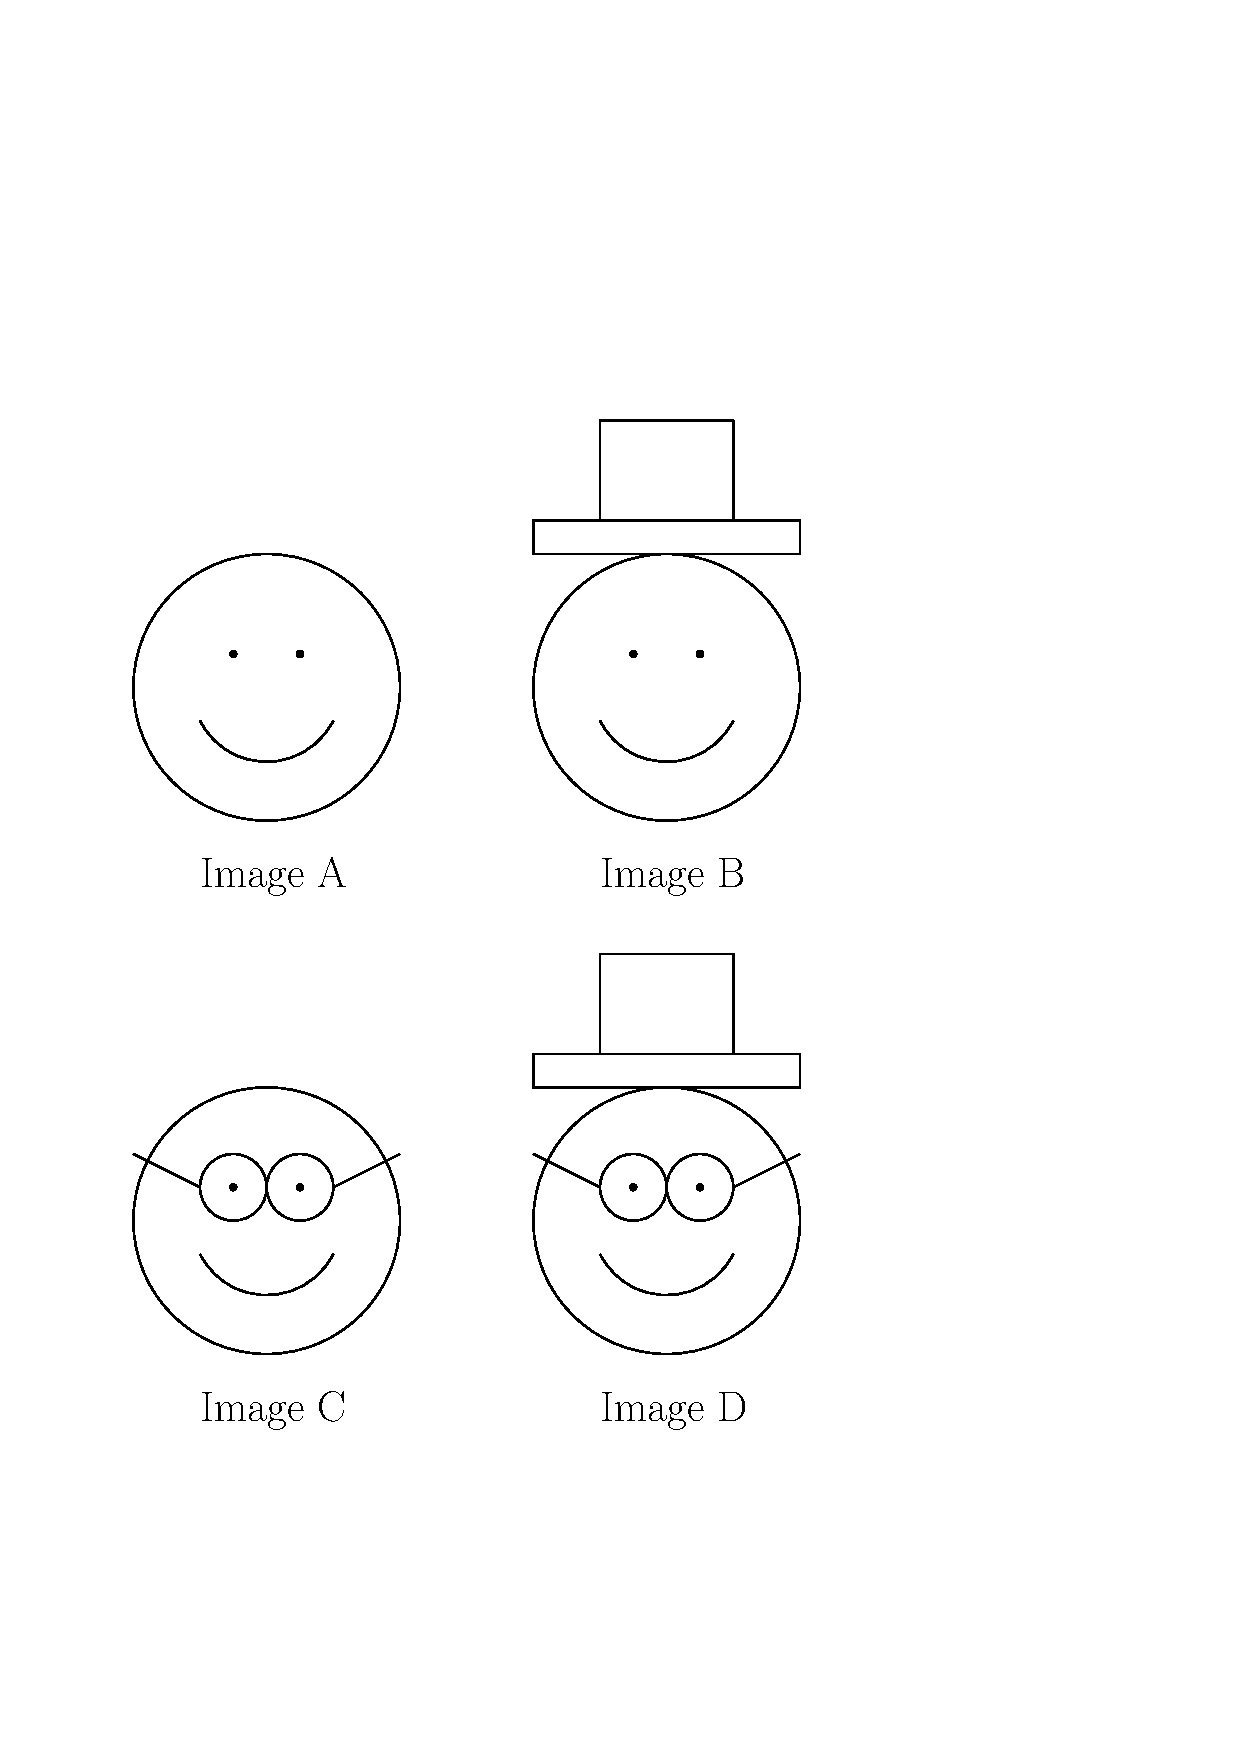
\includegraphics[width=1.5in]{images/TopHatandGlasses.pdf}
\caption{Top Hats and Glasses}\label{fig_tophatandglasses}
\end{center}
\end{figure}
%</truthTables:statement:TopHatAndGlasses:intro>  


%<*truthTables:statement:TopHatAndGlasses:imageP>  
\begin{enumerate}
\item\label{imageP} For which of the images in Figure~{\normalfont\ref{fig_tophatandglasses}} is $P$ true?
%</truthTables:statement:TopHatAndGlasses:imageP>

\Instr{  If $P$ is true then we know that I am wearing a top hat. So $P$ is true in Images B and D.}

\wbvfill
%<*truthTables:statement:TopHatAndGlasses:imageQ>  
\item\label{imageQ} For which of the images in Figure~{\normalfont\ref{fig_tophatandglasses}} is $Q$ true?
%</truthTables:statement:TopHatAndGlasses:imageQ>

\Instr{  If $Q$ is true then we know that I am wearing glasses. So $Q$ is true in images C and D.}
\wbvfill
%<*truthTables:statement:TopHatAndGlasses:imagePandQ>
\item\label{imagePandQ} For which of the images in Figure~{\normalfont\ref{fig_tophatandglasses}} is ``$P$ and $Q$'' true?
%</truthTables:statement:TopHatAndGlasses:imagePandQ>

\Instr{  If ``$P$ and $Q$'' are true, then I am wearing both a top hat and glasses. So ``$P$ and $Q$'' is only true in image D. Students may notice the intersection relationship of Questions~{\normalfont\ref{imageP}} and {\normalfont\ref{imageQ}} to answer this question. We will explore this concept further later in this chapter. We will also eventually consider ``$P$ and $Q$'' to be a single statement; such a statement is true if both $P$ and $Q$ are true, and otherwise is false.}
\wbvfill
%<*truthTables:statement:TopHatAndGlasses:imagePorQ>
\item\label{imagePorQ} For which of the images in Figure {\normalfont\ref{fig_tophatandglasses}} is ``$P$ or $Q$'' true?
%</truthTables:statement:TopHatAndGlasses:imagePorQ>

\Instr{  If ``$P$ or $Q$'' are true, then I am wearing a top hat or I am wearing glasses or I am wearing both. So ``$P$ or $Q$'' is true in images B, C, and D. Students may notice the union relationship of Questions~{\normalfont\ref{imageP}} and {\normalfont\ref{imageQ}}  to answer this question. We will explore this concept further later in this chapter.}

\wbvfill
\end{enumerate}

\newpage

%<*truthTables:statement:TopHatAndGlasses:ActivityTitle>  
\section{Making a Statement}\label{andor}
%</truthTables:statement:TopHatAndGlasses:ActivityTitle>  

\Instr{  Some students may prefer to use manipulatives to solve this problem. Cut out each of the pictures in Figure~{\normalfont\ref{fig_tophatandglasses}} to use as manipulatives.

  
\indent It is important that we be precise about what a statement\index{statement} means in this section. Each statement has the property that it is definitely true or it is definitely false. A statement may change from true to false depending on the group of objects we are considering. For example the statement ``Everyone is at least $16$ years old,'' is likely to be true if we just consider a senior high school class but is false if we consider the entire high school.}

%<*truthTables:statement:TopHatAndGlasses:ActivityAndOr>
\subsection{Activity: Exploring AND and OR Statements}
%</truthTables:statement:TopHatAndGlasses:ActivityAndOr>

%<*truthTables:statement:TopHatAndGlasses:intro4>  
\indent Consider the following statements $P$ and $Q$:
\begin{center}
\begin{tabular}{llc}
$P$: & I am wearing a top hat. & 
\includegraphics[width=.4in]{images/TopHat.pdf}\\
$Q$: & I am wearing glasses. & 
\includegraphics[width=.4in]{images/Glasses.pdf}\\
\end{tabular}
\end{center}

\begin{figure}[htb]
\begin{center}
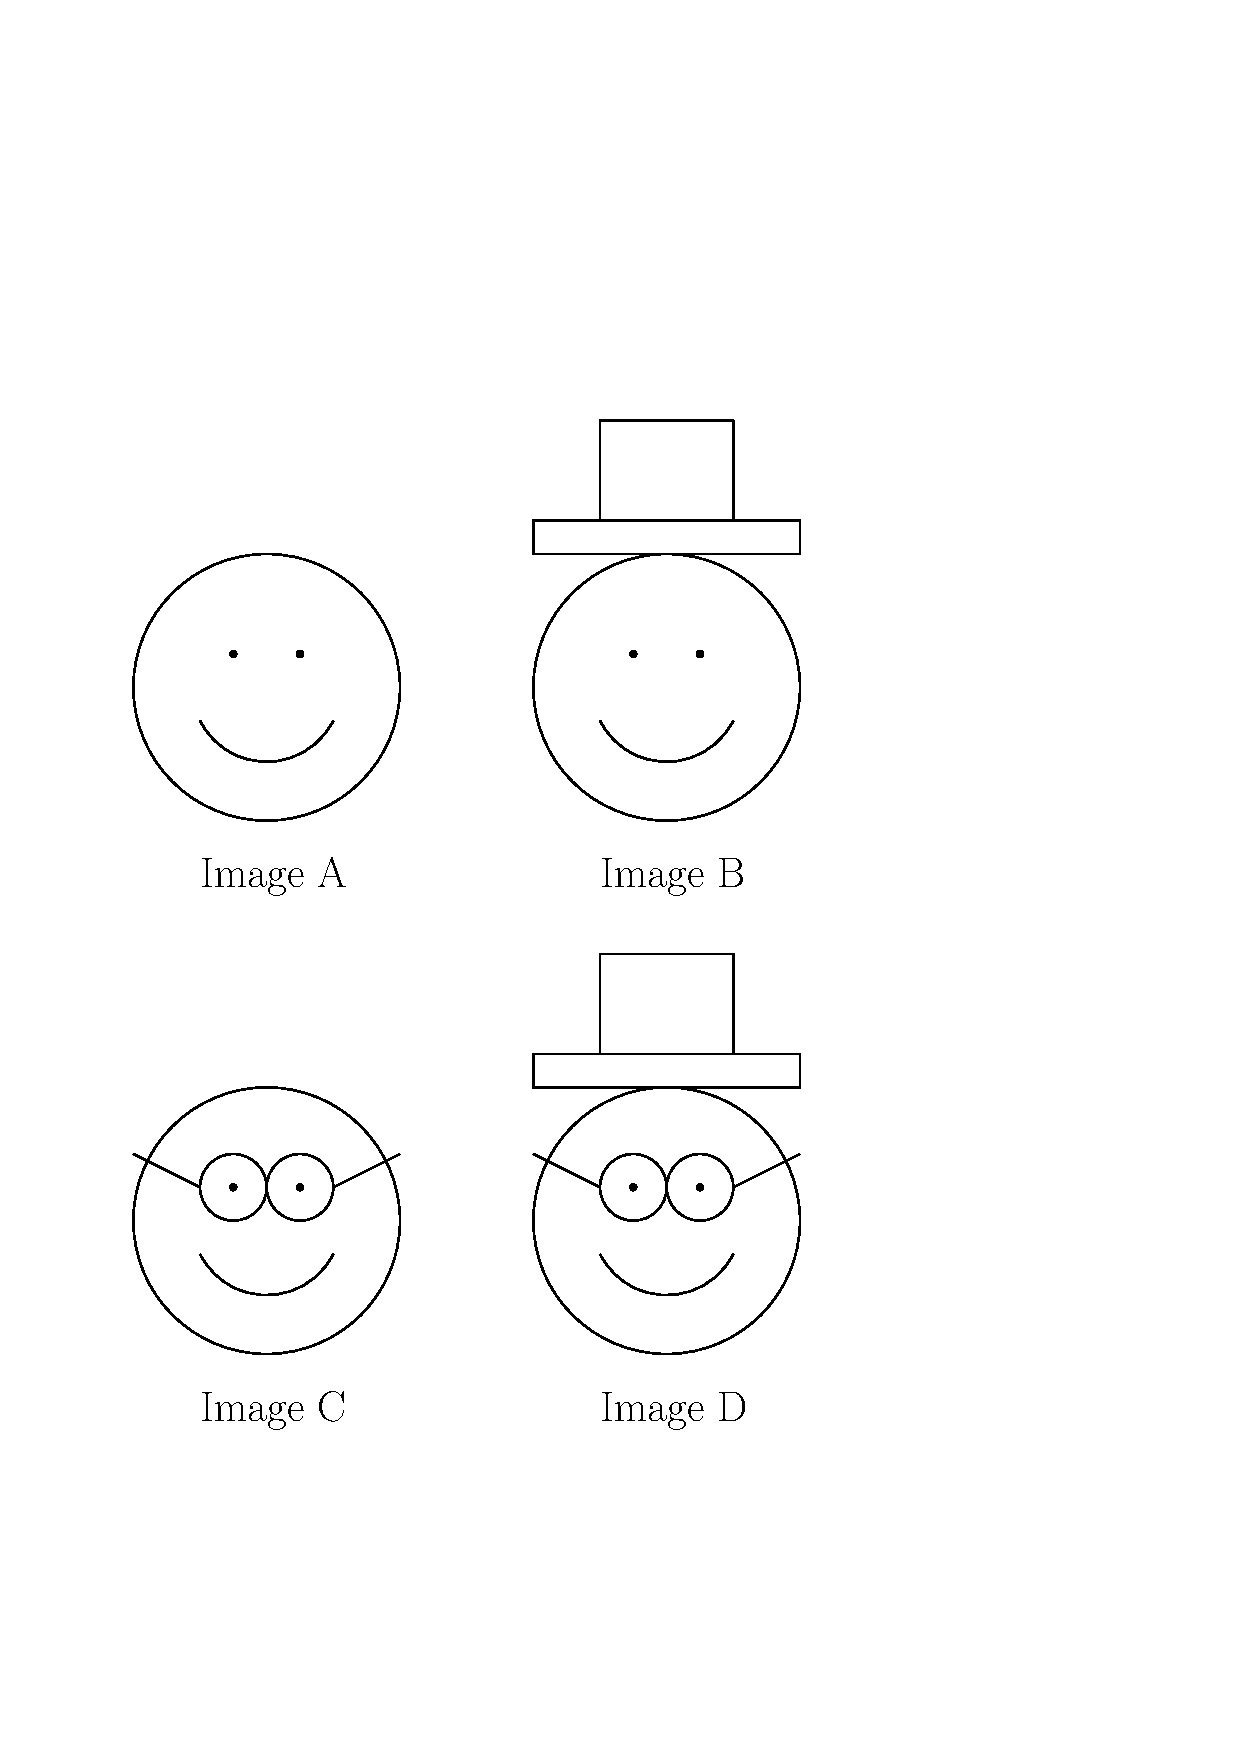
\includegraphics[width=1.5in]{images/TopHatandGlasses.pdf}
\caption{Top Hats and Glasses}\label{fig_tophatandglasses_2}
\end{center}
\end{figure}
%</truthTables:statement:TopHatAndGlasses:intro4>

\begin{enumerate}
%<*truthTables:statement:TopHatAndGlasses:bothPandQtrue>
\item What does it mean when the statement\index{statement} $P$ and the statement $Q$ are both true? Explain what it means if both $P$ and $Q$ are false?
%</truthTables:statement:TopHatAndGlasses:bothPandQtrue>

\Instr{  If $P$ and $Q$ are true, then I am wearing a top hat and glasses at the same time. If $P$ and $Q$ are both false, then I am not wearing a top hat and I am not wearing glasses. Make sure the students precisely understand these statements before moving on to the next question.}
\wbvfill
%<*truthTables:statement:TopHatAndGlasses:topHatNoGlasses>
\item If I am wearing a top hat and no glasses, would the statement\index{statement} ``$P$ and $Q$'' be true or false? Explain your answer.
%</truthTables:statement:TopHatAndGlasses:topHatNoGlasses>

\Instr{  If I am wearing a top hat, then $P$ is true. If I am not wearing glasses then $Q$ is false. So ``$P$ and $Q$'' is false; ``$P$ and $Q$'' being true means that $P$ and $Q$ are both true, so I would be wearing a top hat and glasses.}
\wbvfill

\wbnewpage

%<*truthTables:statement:TopHatAndGlasses:PorQtrue>
\item What would it mean if we knew that the statement\index{statement} ``$P$ or $Q$'' is true? Write out all the possible answers, describing the images in Figure~{\normalfont\ref{fig_tophatandglasses_2}} that make ``$P$ or $Q$'' true.
%</truthTables:statement:TopHatAndGlasses:PorQtrue>

\Instr{  The statement\index{statement} ``$P$ or $Q$'' means that I am wearing a top hat or I am wearing glasses. So there are three possibilities. Make sure the students realize that if I am wearing both a top hat then glasses and the statement ``$P$ or $Q$'' is true. }
\wbvfill

%<*truthTables:statement:TopHatAndGlasses:PorQfalse>
\item What would it mean if we knew that the statement ``$P$ or $Q$'' is false? Write out all the possible answers.
%</truthTables:statement:TopHatAndGlasses:PorQfalse>

\Instr{  If the statement\index{statement} ``$P$ or $Q$'' is false, then I am not wearing a top hat and I am not wearing glasses.}

\wbvfill
%<*truthTables:statement:TopHatAndGlasses:topHatNoGlasses2>
\item If I am wearing a top hat and no glasses, what would you say about the statement ``$P$ or $Q$''; is it true or false?
%</truthTables:statement:TopHatAndGlasses:topHatNoGlasses2>

\Instr{  If I am wearing a top hat and no glasses, then $P$ is true and $Q$ is false. So since $P$ is true, the statement\index{statement} ``$P$ or $Q$'' is true.}

\wbvfill
%<*truthTables:statement:TopHatAndGlasses:4trueFalse>
\item\label{4trueFalse} List all the different ways I can look depending on whether statement $P$ or statement $Q$ is true or false?
%</truthTables:statement:TopHatAndGlasses:4trueFalse>

\Instr{  There are $4$ possibilities: I am wearing a top hat and glasses (both $P$ and $Q$ are true), I am wearing a top hat but I am not wearing glasses ($P$ is true and $Q$ is false), I am not wearing a top hat but I am wearing glasses ($P$ is false and $Q$ is true), and I am not wearing a top hat or glasses (both $P$ and $Q$ are false).}
\wbvfill
%<*truthTables:statement:TopHatAndGlasses:end>
\end{enumerate}
%</truthTables:statement:TopHatAndGlasses:end>

\newpage

%<*truthTables:statement:tophat:intro>
\subsection{Activity: Top Hats, Overalls, and Rain boots}\label{tophat}
%</truthTables:statement:tophat:intro>

\Instr{  
Goals for this activity:
\begin{packedItem}
\item Developing situations for given compound statements; and
\item Completing Truth Tables for compound statements.
\end{packedItem}
}

%<*truthTables:statement:tophat:intro2>
\indent Let $P\wedge Q$\index{$\wedge$} be the single statement ``$P$ and $Q$'' and let $P\vee Q$\index{$\vee$} be the single statement ``$P$ or $Q$.'' Consider the statements below:
\begin{center}
\begin{tabular}{ll}
$P$: & I am wearing a top hat.\\
$Q$: & I am wearing overalls.\\
$R$: & I am wearing rain boots.\\
\end{tabular}
\end{center}

\begin{enumerate}
\setcounter{enumi}{6}
\item What do I look like if $P\wedge Q$ is true? Am I wearing the same thing if $Q\wedge P$ is true? 
%</truthTables:statement:tophat:intro2>

\Instr{  If the statement $P\wedge Q$ is true then I must be wearing both atop hat and overalls, but I may or may not be wearing rain boots. So there are two possible answers. Since $Q\wedge P$ being true means  that I am wearing overalls and a top hat, this scenario has the same two possible answers. So I may be wearing different things (i.e. ``top hat, overalls and boots'' or ``overalls, top hat, but not boots''). But since the sets of answers are the same, we say that the statement\index{statement} $P\wedge Q$ is equivalent to statement $Q\wedge P$\index{$\wedge$}.

The students may want to answer this question by ignoring $R$ completely. In such a case there is only one answer in both cases: I am wearing a top hat and overalls.}

\wbvfill
%<*truthTables:statement:tophat:PwedgeQfalse>
\item What do I look like if $P\wedge Q$ is false? Is there more than one answer? If so, list out all the possible ways I could be dressed.
%</truthTables:statement:tophat:PwedgeQfalse>

\Instr{  The students may or may not include rain boots in these answers considering that the question does not mention statement $R$. Both methods answers are correct and could be discussed as a class. If $P\wedge Q$ is false, then it is not the case that I am wearing both a top hat and overalls. Therefore, I could be wearing the overalls but not the top hat, I could be wearing a top hat but not overalls, or the only other way to be dressed would be if I can not wearing overalls and I can not wearing a top hat. So if $R$ is ignored then there are $3$ possible answers. If boots are considered by the students then each of the $3$ answers can be extended by either having me in boots or not, so then there are $6$ answers.}

\wbvfill

%<*truthTables:statement:tophat:PveeQtrue>
\item What am I wearing if $P\vee Q$\index{$\vee$} is true? Is there any difference in my outfit if $Q\vee P$ is true? List all possible outfits that make these statements\index{statement} true.
%</truthTables:statement:tophat:PveeQtrue>

\Instr{  The statement $P\vee Q$ means that I am wearing a top hat or I am wearing overalls, so I can be wearing only the top hat and not the overalls, I can be wearing overalls and not the top hat, or I can be wearing both the top hat and the overalls. All of these answers can be written with or without rain boots, giving a total of $3$ possible solutions if the students do not include the rain boots in the problem  and $6$ possible solutions otherwise. 

As before, there is no difference between the set of answers that make the statements $P\vee Q$ and $Q\vee P$ true, so they are equivalent.}

\wbvfill
%<*truthTables:statement:tophat:logicTable>
\item\label{logicTable} Fill in the table below. Each cell in the table should contain either ``True'' or ``False.'' First write in all the possible truth values for the pair of statements\index{statement} $P$ and $Q$ in the first two columns (see Question~{\normalfont\ref{4trueFalse}} for some help). Then in the third and fourth columns describe how $P\wedge Q$\index{$\wedge$} and $P\vee Q$\index{$\vee$} will be affected by your choice of $P$ and $Q$ in the corresponding row. This table is called a truth table\index{truth table}.
\begin{center}
\begin{tabular}{|c|c||c|c|}
\hline
$P$ & $Q$ & $P\wedge Q$ & $P\vee Q$ \\
\hline
\hline
\hspace{.75in} & \hspace{.75in} & \hspace{.75in} & \hspace{.75in} \\
\hline
 &  & & \\
\hline
 & & & \\
\hline
 & & & \\
\hline
\end{tabular}
\end{center}
%</truthTables:statement:tophat:logicTable>

\Instr{ 
The order in which the rows are listed in the following table is not important.
\begin{center}
\begin{tabular}{|c|c||c|c|}
\hline
$P$ & $Q$ & $P\wedge Q$ & $P\vee Q$ \\
\hline
\hline
True & True & True & True \\
\hline
True & False & False & True \\
\hline
False & True & False & True \\
\hline
False & False & False & False \\
\hline
\end{tabular}
\end{center}
}

\wbnewpage

%<*truthTables:statement:tophat:PandQandR2>
\item\label{PandQandR2} What do I look like if $P\wedge Q\wedge R$ is true? 
%</truthTables:statement:tophat:PandQandR2>

\Instr{  If $P\wedge Q\wedge R$ is true then I am wearing a top hat and overalls and rain boots. There is only one possible answer.}
\wbvfill
%<*truthTables:statement:tophat:order?>
\item Does my outfit change if we reorder $P$, $Q$, and $R$ in Question~{\normalfont\ref{PandQandR2}}? Explain your answer.
%</truthTables:statement:tophat:order?>

\Instr{  No matter the order of the articles that I am wearing, the statements\index{statement} $P\wedge Q\wedge R$\index{$\wedge$}, $P\wedge R\wedge Q$, $R \wedge P \wedge Q$, $R\wedge Q\wedge P$, $Q\wedge P \wedge R$, and $Q\wedge R\wedge P$ are all equivalent. The reason for this is because for $P\wedge Q\wedge R$ to be true, the statements $P$, $Q$, and $R$ must all be true. If any one of these statements are false then $P\wedge Q \wedge R$ is false.}
\wbvfill
%<*truthTables:statement:tophat:describePorQandR>
\item\label{describePorQandR} Describe my clothing if $(P\vee Q) \wedge R$ is true. List out all the possible clothing options. \Hint{ There are three.}
%</truthTables:statement:tophat:describePorQandR>

\Instr{  The statement\index{statement} $(P\vee Q)\wedge R$\index{$\vee$} means that I am wearing a top hat and rain boots, I am wearing overalls and rain boots, or I am wearing a top hat, overalls, and rain boots. If this statement is true, then notice that $R$ must be true and $P\vee Q$ must be true. Thus I must be wearing rain boots, and I must be wearing overalls or a top hat.
}
\wbvfill
%<*truthTables:statement:tophat:describePorQandR2>
\item\label{describePorQandR2} Describe my clothing if $P\vee (Q\wedge R)$ is true. List out all the possible clothing options. \Hint{ There are five.}
%</truthTables:statement:tophat:describePorQandR2>

\Instr{  The statement\index{statement} $P\vee (Q\wedge R)$\index{$\vee$}\index{$\wedge$} says I am wearing a top hat, I am wearing overalls and rain boots, or I am wearing a top hat, overalls, and rain boots.}
\wbvfill
%<*truthTables:statement:tophat:describePorQandR3>

\wbnewpage
\item\label{describePorQandR3} Fill in the table below. Each cell in the table should contain either ``True'' or ``False.'' As in Question~{\normalfont\ref{logicTable}} first fill in the first three columns so that no two rows have exactly the same three truth values for $P$, $Q$ and $R$. The your choice of $P$, $Q$, and $R$ in each row will determine the truth value in the next three columns. \Hint{ see questions~{\normalfont\ref{describePorQandR}} and~{\normalfont\ref{describePorQandR2}}.}
\begin{center}
\begin{tabular}{|c|c|c||c|c|}
\hline
$P$ & $Q$ & $R$ & $(P\vee Q) \wedge R$ & $P\vee (Q \wedge R)$ \\
\hline
\hline
\hspace{.75in} & \hspace{.75in} & \hspace{.75in} & \hspace{.75in} & \hspace{.75in} \\
\hline
 & & & & \\
\hline
 & & & & \\
\hline
 & & & & \\
\hline
 & & & & \\
\hline
 & & & & \\
\hline
 & & & & \\
\hline
 & & & & \\
\hline
\end{tabular}
\end{center}
%</truthTables:statement:tophat:describePorQandR3>

\Instr{  
The order of the rows in the following table is not important.
\begin{center}
\begin{tabular}{|c|c|c||c|c|}
\hline
$P$ & $Q$ & $R$ & $(P\vee Q) \wedge R$ & $P\vee (Q \wedge R)$ \\
\hline
\hline
True & True & True & True & True \\
\hline
True & True & False & False & True \\
\hline
True & False & True & True & True \\
\hline
True & False & False & False & True \\
\hline
False & True & True  & True & True \\
\hline
False & True & False & False & False \\
\hline
False & False & True & False & False \\
\hline
False & False & False & False & False \\
\hline
\end{tabular}
\end{center}
}
%<*truthTables:statement:tophat:describePorQandR4>
\item Using the truth table\index{truth table} in Question~{\normalfont\ref{describePorQandR3}} determine if the statement\index{statement} $P\vee (Q\wedge R)$\index{$\vee$}\index{$\wedge$} the same as the statement $(P\vee Q)\wedge R$. Explain yourself thoroughly.
%</truthTables:statement:tophat:describePorQandR4>

\Instr{  Just by reading over the meanings of these statements it is clear that $(P\vee Q)\wedge R$ is not the same as $P\vee (Q\wedge R)$. The truth table in Question~{\normalfont\ref{describePorQandR3}} also tells us the same conclusions that when $P$ is true and $R$ is false, the two statements are not equivalent regardless of the truth value for $Q$.}

\wbvfill
%<*truthTables:statement:tophat:PandQandR>
\item\label{PandQandR} Suppose I am wearing a top hat and rain boots, and I am not wearing overalls. Is the statement\index{statement} $(P\wedge Q) \wedge R$\index{$\wedge$}\index{$\vee$} true or false? Is the statement $(P\wedge R) \vee Q$ true or false?
%</truthTables:statement:tophat:PandQandR>

\Instr{  According to the question given, $P$ is true, $Q$ is false, and $R$ is true. Since $P\wedge Q$ is false, $(P\wedge Q)\wedge R$ is false. Similarly, since $P\wedge R$ is true, $(P\wedge R) \vee Q$ is true.}

\wbvfill
\end{enumerate}

\newpage

\subsection{Exit Slip}

%<*truthTables:statement:tophat:logicTable2>
 Fill in the table below. Each cell in the table should contain either ``True'' or ``False.'' As in Question~{\normalfont\ref{logicTable}}, begin by completing the first three columns.
\begin{center}
\begin{tabular}{|c|c|c||c|c|c|}
\hline
$P$ & $Q$ & $R$ & $(P\wedge Q) \wedge R$ & $(P\vee Q) \vee R$ & $P\vee (Q \wedge R)$ \\
\hline
\hline
\hspace{.75in} & \hspace{.75in} & \hspace{.75in} & \hspace{.75in} & \hspace{.75in} & \hspace{.75in} \\
\hline
 & & & & & \\
\hline
 & & & & & \\
\hline
 & & & & & \\
\hline
 & & & & & \\
\hline
 & & & & & \\
\hline
 & & & & & \\
\hline
 & & & & & \\
\hline
\end{tabular}
\end{center}
%</truthTables:statement:tophat:logicTable2>

\Instr{  
\begin{center}
\begin{tabular}{|c|c|c||c|c|c|}
\hline
$P$ & $Q$ & $R$ & $(P\wedge Q) \wedge R$ & $(P\vee Q) \vee R$ & $P\vee (Q \wedge R)$ \\
\hline
\hline
True & True & True & True & True & True \\
\hline
True & True & False & False & True & True \\
\hline
True & False & True & False & True & True \\
\hline
True & False & False & False & True & True \\
\hline
False & True & True & False & True & True \\
\hline
False & True & False & False & True & False \\
\hline
False & False & True & False & True & False \\
\hline
False & False & False & False & False & False \\
\hline
\end{tabular}
\end{center}
}
%<*truthTables:statement:tophat:end>
%</truthTables:statement:tophat:end>

%<*truthTables:statement:tophat:exit>


%</truthTables:statement:tophat:exit>
\newpage

%<*truthTables:statement:negation:intro>
\subsection{Activity: Negation}\label{negation}
%</truthTables:statement:negation:intro>

\Instr{  
Goals for this activity:
\begin{packedItem}
\item Working with negations withing compound statements; 
\item Determining truth values of compound statements containing negations; 
\item Completing Truth Tables for compounstatements containing negations; and
\item Determining weather two statements are equivalent.
\end{packedItem}
}

%<*truthTables:statement:negation:intro2>
\indent Let $\neg P$ represent the statement\index{statement} ``not $P$''. For example, if $P$ represents the statement "It is raining." then $\neg P$ represents the statement "It is not raining." $\neg P$\index{$\neg$} is called the negation of $P$. Again we will consider the statements below.
\begin{center}
\begin{tabular}{ll}
$P$: & I am wearing a top hat.\\
$Q$: & I am wearing overalls.\\
$R$: & I am wearing rain boots.\\
\end{tabular}
\end{center}

\begin{enumerate}
\setcounter{enumi}{26}
\item\label{negPtrue} If $\neg P$ is true, is anything on my head? 
%</truthTables:statement:negation:intro2>

\Instr{  When $\neg P$ is true, ``$P$ is false'' is true, so I am not wearing a top hat. So there maybe something on my head, but it is not a top hat!}

\wbvfill
%<*truthTables:statement:negation:negPtrue>
\item If $\neg P$ is false, is anything on my head?
%</truthTables:statement:negation:negPtrue>

\Instr{  When $\neg P$ is false, ``$P$ is false'' is false, so $P$ is true. Therefore there is something on my head when $\neg P$ is false, namely a top hat.}
\wbvfill
%<*truthTables:statement:negation:negPfalse>
\item Fill in the truth table\index{truth table} below. Each cell in the table should contain either ``True'' or ``False.'' As in Question~{\normalfont\ref{logicTable}} begin by completing the first column.
\begin{center}
\begin{tabular}{|c||c|}
\hline
$P$ & $\neg P$ \\
\hline
\hline
\hspace{.75in} & \hspace{.75in} \\
\hline
& \\
\hline
\end{tabular}
\end{center}
%</truthTables:statement:negation:negPfalse>

\Instr{  
\begin{center}
\begin{tabular}{|c||c|}
\hline
$P$ & $\neg P$ \\
\hline
\hline
True & False \\
\hline
False & True \\
\hline
\end{tabular}
\end{center}
}

%<*truthTables:statement:negation:PwedgeRfalse>
\item Suppose you know the statement $P\wedge R$\index{$\wedge$} is false. Describe what I'm wearing. Is there a statement that says the same thing when it is true?
%</truthTables:statement:negation:PwedgeRfalse>

\Instr{  If $P\wedge R$ is false then it is not the case that I am wearing both a top hat and rain boots. Therefore I am either ``not wearing a top hat'' or ``I am not wearing rain boots.'' The easiest way to find a corresponding true statement is to simply apply the $\neg$ function and use $\neg (P\wedge R)$. But the verbal description of what I'm wearing leads to another solution: $\neg P \vee \neg Q$\index{$\neg$}\index{$\vee$}. Encourage the students to find both answers.}

\wbvfill

\newpage

%<*truthTables:statement:negation:QveeRfalse>
\iffalse
\item Suppose you know the statement $Q\vee R$ is false. Describe what I'm wearing. Is there a statement\index{statement} that says the same thing when it is true?
%</truthTables:statement:negation:QveeRfalse>

\Instr{  If $Q\vee R$ is false then it is not the case that either I am wearing overalls or I am wearing rain boots. So I cannot be wearing either. Therefore I am not wearing overalls and I am not wearing rain boots. So both the statement\index{statement} $\neg Q \wedge \neg R$\index{$\neg$}\index{$\wedge$} is true. What I am wearing is also described by $\neg(Q\wedge R)$, as can be seen by applying the definition of $\neg$. So both are good answers.}

%<*truthTables:statement:negation:PwedgenegQfalse>
\item Suppose you know that statement $P\wedge \neg Q$ is false. Describe what I'm wearing. Is there a statement that says the same thing when it is true?
%</truthTables:statement:negation:PwedgenegQfalse>

\Instr{  If $P\wedge \neg Q$ is false then it is not the case that I am both wearing a top hat and not wearing overalls. Therefore either I am not wearing a top hat or I am wearing overalls. So the statement\index{statement} $\neg P\vee Q$\index{$\neg$}\index{$\vee$}\index{$\wedge$} is true. Also, $\neg(P\wedge \neg Q)$ is true by the definition of $\neg$. So both are good answers.}
\fi
%<*truthTables:statement:negation:logicTable2.5>
\item\label{logicTable2.5} Fill in the truth table\index{truth table} below so that each cell contains either ``True'' or ``False.'' As in Question~{\normalfont\ref{logicTable}}, begin by completing the first two columns so that all ways truth values can be assigned to $P$ and $Q$ are represented in the four rows.
\begin{center}
\begin{tabular}{|c|c||c|c|c|c|}
\hline
$P$ & $Q$ & $\neg P$ & $\neg Q$ & $\neg(P\wedge Q)$ & $\neg P\vee \neg Q$ \\
\hline
\hline
\hspace{.5in} & \hspace{.5in} & \hspace{.5in} & \hspace{.5in} & \hspace{.75in} & \hspace{.75in} \\
\hline
&&&&& \\
\hline
&&&&& \\
\hline
&&&&& \\
\hline
\end{tabular}
\end{center}
%</truthTables:statement:negation:logicTable2.5>

\Instr{ 
\begin{center}
\begin{tabular}{|c|c||c|c|c|c|}
\hline
$P$ & $Q$ & $\neg P$ & $\neg Q$ & $\neg (P\wedge Q)$ & $\neg P\vee \neg Q$ \\
\hline
\hline
True & True & False & False & False & False  \\
\hline
True & False & False & True & True & True  \\
\hline
False & True & True & False & True & True \\
\hline
False & False & True & True & True & True \\
\hline
\end{tabular}
\end{center}
}

%<*truthTables:statement:negation:sameStatement?>
\item Using the truth table\index{truth table} in Question~{\normalfont\ref{logicTable2.5}} determine if the statement $\neg(P\wedge R)$ is the same as the statement\index{statement}\index{$\wedge$}\index{$\vee$}\index{$\neg$} $\neg P \vee \neg R$. Explain yourself thoroughly.
%</truthTables:statement:negation:sameStatement?>

\Instr{  Based on the truth table they are the same. Also, by reasoning out what each of the statements is saying, it is clear that the two statements are identical.}

\iffalse
%<*truthTables:statement:negation:logicTable3>
\item\label{logicTable3} Fill in the table below so that each cell contains either ``True'' or ``False.'' As in Question~{\normalfont\ref{logicTable}}, begin by completing the first two columns.
\begin{center}
\begin{tabular}{|c|c||c|c|c|c|c|}
\hline
$P$ & $Q$ & $\neg P$ & $\neg Q$ & $\neg P\wedge Q$ & $P\vee \neg Q$ & $\neg P\vee \neg Q$ \\
\hline
\hline
\hspace{.5in} & \hspace{.5in} & \hspace{.5in} & \hspace{.5in} & \hspace{.75in} & \hspace{.75in} & \hspace{.75in} \\
\hline
&&&&&& \\
\hline
&&&&&& \\
\hline
&&&&&& \\
\hline
\end{tabular}
\end{center}
%</truthTables:statement:negation:logicTable3>

\Instr{  
\begin{center}
\begin{tabular}{|c|c||c|c|c|c|c|}
\hline
$P$ & $Q$ & $\neg P$ & $\neg Q$ & $\neg P\wedge Q$ & $\neg P\vee \neg Q$ & $P\vee \neg Q$ \\
\hline
\hline
True & True & False & False & False & False & True \\
\hline
True & False & False & True & False & True & True \\
\hline
False & True & True & False & True & True & False \\
\hline
False & False & True & True & False & True & True \\
\hline
\end{tabular}
\end{center}
}
\fi

\wbvfill
%<*truthTables:statement:negation:logicTable4>
\item\label{logicTable4} Fill in the table below so that each cell contains either ``True'' and ``False.'' As in Question~{\normalfont\ref{logicTable}}, begin by completing the first three columns.
\begin{center}
\begin{tabular}{|c|c|c||c|c|c|}
\hline
$P$ & $Q$ & $R$ & $(P\wedge Q) \wedge \neg R$ & $(\neg P \vee \neg Q) \vee R$ & $(P\vee \neg Q) \wedge \neg R$ \\
\hline
\hline
\hspace{.44in} & \hspace{.44in} & \hspace{.44in} &&& \\
\hline
&&&&& \\
\hline
&&&&& \\
\hline
&&&&& \\
\hline
&&&&& \\
\hline
&&&&& \\
\hline
&&&&& \\
\hline
&&&&& \\
\hline
\end{tabular}
\end{center}
%</truthTables:statement:negation:logicTable4>

\Instr{  
\begin{center}
\begin{tabular}{|c|c|c||c|c|c|}
\hline
$P$ & $Q$ & $R$ & $(P\wedge Q) \wedge \neg R$ & $(\neg P \vee \neg Q) \vee R$ & $(P\vee \neg Q) \wedge \neg R$ \\
\hline
\hline
True & True & True & False & True & False \\
\hline
True & True & False & True & False & True \\
\hline
True & False & True & False & True & False \\
\hline
True & False & False & False & True & True \\
\hline
False & True & True & False & True & False \\
\hline
False & True & False & False & True & False \\
\hline
False & False & True & False & True & False \\
\hline
False & False & False & False & True & True \\
\hline
\end{tabular}
\end{center}
}


%<*truthTables:statement:negation:end>
\end{enumerate}
%</truthTables:statement:negation:end>

\newpage

\subsection{Activity: The Implications\index{implication} of Your Actions}\label{implications}
%</truthTables:implications:title>

\Instr{  
Goals for this activity:
\begin{packedItem}
\item Making truth tables for implication statements; 
\item Writing symbolic statements which represent a given written statements; and
\item Creating equivalent statements using implication conjunctions.
\end{packedItem}
}

%<*truthTables:implications:intro>
The last activity introduced the basic form of an argument used by mathematicians. They assume that something is true and then see if that means whether you know other things are true. This step is called an \textbf{implication}\index{implication}. We say that ``$P$ implies $Q$'', and write $P\Rightarrow Q$, if whenever $P$ is true $Q$ is also true. So the only way that the statement\index{statement} $P\Rightarrow Q$\index{$\wedge$} can be false is when $P$ is true and $Q$ is false. 

\begin{enumerate}
\item Consider the statement ``If it's Monday, my day will suck.'' This is an implication where $P = $ ``today is Monday'' and $Q = $ ``I will have a sucky day today.''  Discuss with your group members:  What are the 4 possible options for T/F for $P$ and $Q$.  In which of those scenarios is the person who claims ``If it's Monday, my day will suck'' saying something true?  In which scenario are they wrong?

\wbvfill

\item\label{implyTable} Fill in the following table so that each cell contains either ``True'' or ``False.'' First write in all the possible truth values for the pair of statements $P$ and $Q$ in the first two columns. Then in the third column indicate how $P\Rightarrow Q$ will be affected by your choice of $P$ and $Q$ in the corresponding row. 

\begin{center}
\begin{tabular}{|c|c||c|}
\hline
$P$ & $Q$ & $P\Rightarrow Q$ \\
\hline
\hline
\hspace{.4in} & \hspace{.4in} & \hspace{.4in}  \\
\hline
&& \\
\hline
&& \\
\hline
&& \\
\hline
\end{tabular}
\end{center}
%</truthTables:implications:intro>

\Instr{  The students may not know what to fill in for $P\Rightarrow Q$\index{$\Rightarrow$} when $P$ is false. Point them to the definition where it says there is only one way to make $P\Rightarrow Q$ false.
\begin{center}
\begin{tabular}{|c|c||c|}
\hline
$P$ & $Q$ & $P\Rightarrow Q$ \\
\hline
\hline
True & True & True \\
\hline
True & False & False \\
\hline
False & True & True \\
\hline
False & False & True \\
\hline
\end{tabular}
\end{center}
}

%<*truthTables:implications:PimpliesQ>
\item Notice that $P\Rightarrow Q$ is always true whenever $P$ is false. Why do you think that is the case?
%</truthTables:implications:PimpliesQ>

\Instr{  $P\Rightarrow Q$ only tries to assert something about $Q$ when $P$ is itself true. If $P$ is false, then $P\Rightarrow Q$ is not trying to assert anything, so it cannot be false.
}

\wbvfill

\wbnewpage

%<*truthTables:implications:tuesdayRaining>
\item Suppose the statement\index{statement} ``If it is Tuesday then it must be raining all day'' is true. What do you know if:
\begin{enumerate}
\item it is not raining outside.
\wbvfill

\item it is Tuesday today.
\wbvfill
\item it is Wednesday today.
\wbvfill
\end{enumerate}
%</truthTables:implications:tuesdayRaining>

\Instr{  \begin{enumerate}
\item It cannot be Tuesday (because on Tuesday it is raining).
\item It is raining all day today.
\item We do not know anything about the weather. It is worth asking the students to assign a letter to the two statements in the implication\index{implication}, say
\begin{center}
\begin{tabular}{ll}
$T$: & It is Tuesday. \\
$R$: & It is raining all day. \\
\end{tabular}
\end{center}
Then ask the students

\begin{minipage}[H]{5.75in}
\tt \em
\begin{center}
{``What are we told is true?''}
\end{center}
\end{minipage}

We know $T\Rightarrow R$ is true. Then ask

\begin{minipage}[H]{5.75in}
\tt \em
\begin{center}
{``What does each of (a), (b), and (c) tell us about the truth value of $T$ and $R$?''}
\end{center}
\end{minipage}

and then

\begin{minipage}[H]{5.75in}
\tt \em
\begin{center}
{``How does this help you answer the question?''}
\end{center}
\end{minipage}

To this you can answer
\begin{enumerate}
\item[(a)] $R$ is false. But $T\Rightarrow R$ is true. So from the table in Question~{\normalfont\ref{implyTable}} we know that $T$ must be false.
\item[(b)] $T$ is true. But $T\Rightarrow R$ is also true. So from the table in Question~{\normalfont\ref{implyTable}} $R$ must be true.
\item[(c)] $T$ is false. So from the table in Question~{\normalfont\ref{implyTable}}, $R$ could be true or false.
\end{enumerate}
\end{enumerate}
}

%<*truthTables:implications:endRainUmbrella>
\end{enumerate}		

\newpage
Consider the statements below for Questions~{\normalfont\ref{P->Q}}--{\normalfont\ref{P->RandS}}.
\begin{center}
\begin{tabular}{ll}
$P$: & It is raining today. \\
$Q$: & I bring an umbrella with me. \\
$R$: & I play basketball during recess. \\
$S$: & I took a test in English class. \\
\end{tabular}
\end{center}

\begin{enumerate}
\setcounter{enumi}{4}
\item\label{P->Q} Write the statement

\begin{minipage}[H]{5.75in}
\tt \em 
\begin{center}
{``If it is raining today then I will bring an umbrella with me.''}
\end{center}
\end{minipage}

\noindent using the symbolic statements $P$, $Q$, $R$, and $S$. Explain why you know your answer is correct.
%</truthTables:implications:endRainUmbrella>

\Instr{  This is to make sure the students have a understanding of symbolic statements of implications\index{implication}. The answer should be $P \Rightarrow Q$\index{$\Rightarrow$}. }

\wbvfill

\iffalse
%<*truthTables:implications:P->P>
\item\label{P->P} Write the statement\index{statement}

\begin{minipage}[H]{5.75in}
\tt \em
\begin{center}
{``If it is raining today then it is raining today.'' }
\end{center}
\end{minipage}

\noindent using the symbolic statements $P$, $Q$, $R$, and $S$. Explain why you know your answer is correct.
%</truthTables:implications:P->P>

\Instr{  The answer is $P \Rightarrow P$. This is a good time to have students really think about what they are writing. This statement seems a bit trivial intact it is always true. We will explore other statements that are always true that do not seem as trivial later.}

\fi
%<*truthTables:implications:P->RandS>
\item\label{P->RandS} Write the statement\index{statement}

\begin{minipage}[H]{5.75in}
\tt \em
\begin{center}
{``If it is raining today then I will play basketball and take a test in English class.''}
\end{center}
\end{minipage}

\noindent using the symbolic statements $P$, $Q$, $R$, and $S$. Explain why you know your answer is correct.
%</truthTables:implications:P->RandS>

\Instr{   This is a time when we must discuss how the order and wording of a sentence can affect the symbolic statements. This statement seems to have two possible answers if one does not technically define what is meant by the statement. The confusion is derived when we we consider the ``and'' portion of the statement.

 We must decide weather the ``and'' statement\index{statement} is applied inside the implication or if the implication\index{implication} is applied inside the ``and'' statement. Students may write the statement as $(P\Rightarrow R) \wedge S$\index{$\wedge$}, but there is a subtlety in the fact that there is only one ``I will'' in the statement therefore providing a clue that the statement is intended to be $P \Rightarrow (R \wedge S)$ because the statement infers that if it is raining then we will do both of the following (play basketball and take the test.
 
 This might be a good time to discuss ordering of sentences. If we wanted to mean $(P\Rightarrow R) \wedge S$ it is possible to place another ``I will'' after the ``and'' in the above sentence but better than that we can reorder the sentence. This is possible since the ``and'' conjunction is associative. So we would write ``I will take a test in English class  and If it is raining today then I will play basketball.'' which is symbolically written as $S \wedge (P\Rightarrow R)$\index{$\Rightarrow$} and obviously equivalent to  $(P\Rightarrow R) \wedge S$}

\wbvfill
\iffalse
%<*truthTables:implications:RorQ->P>
\item \label{RorQ->P} Write the statement\\
\begin{minipage}[H]{5.75in}
\tt \em 
\begin{center}
{``If I play basketball today or I brought my umbrella with me then it is raining today.''}
\end{center}
\end{minipage}\\
using the symbolic statements\index{statement} $P$, $Q$, $R$, and $S$. Explain why you know your answer is correct.
%</truthTables:implications:RorQ->P>

\Instr{  Again we have combined previously mentioned conjunctions with an implication\index{implication}, but here there should be no issue to which statement is inside the other, however if we are not careful with our use of parenthesis we could write a symbolic statement which is not indicative of the statement which is written. The students should be written as $(R \vee Q) \Rightarrow P$\index{$\vee$}\index{$\Rightarrow$}. But it should be noted that if we leave the parenthesis off we have written a symbolic statement where the implication\index{implication} is inside the ``or'' statement, which is not an accurate representation of the statement given.}

\fi
%<*truthTables:implications:implicationsTable>
\item\label{implicationsTable} Fill in Table~{\normalfont\ref{implicationsTable1}} so that each cell contains either ``True'' or ``False.'' First write in all the possible truth values for the pair of statements $P$ and $Q$ in the first two columns. Then in the remaining columns indicate how the other statements will be affected by your choice of $P$ and $Q$ in the corresponding row.

\index{$\neg$}\index{$\Rightarrow$}
\begin{table}[htb]
\begin{center}
\begin{tabular}{|c|c||c|c|c|c|c|c|}
\hline
\strut $P$ & $Q$ & $\neg P$ & $\neg Q$ & $P\Rightarrow Q$ & $Q\Rightarrow P$ & $\neg P \Rightarrow \neg Q$ & $\neg Q \Rightarrow \neg P$\\
\hline
\hline
\strut \hspace{.4in} & \hspace{.4in} & \hspace{.4in} & \hspace{.4in} & \hspace{.7in} & \hspace{.7in} & \hspace{.7in} & \hspace{.7in}  \\
\hline
\strut&&&&&&& \\
\hline
\strut&&&&&&& \\
\hline
\strut&&&&&&& \\
\hline
\end{tabular}
\caption{Table of logical statements\index{statement} using the $\Rightarrow$ symbol}\label{implicationsTable1}
\end{center}
\end{table}
%</truthTables:implications:implicationsTable>

\wbnewpage

\Instr{ 
\begin{center}
\begin{tabular}{|c|c||c|c|c|c|c|c|}
\hline
$P$ & $Q$ & $\neg P$ & $\neg Q$ & $P\Rightarrow Q$ & $Q\Rightarrow P$ & $\neg P \Rightarrow \neg Q$ & $\neg Q \Rightarrow \neg P$\\
\hline
\hline
True&True&False&False&True&True&True&True \\
\hline
True&False&False&True&False&True&True&False \\
\hline
False&True&True&False&True&False&False&True \\
\hline
False&False&True&True&True&True&True&True \\
\hline
\end{tabular}
\end{center}
}

%<*truthTables:implications:P->QTrue>
\item If $P\Rightarrow Q$ is true, does that mean that $Q\Rightarrow P$ is true. Give a justification for your answer.
%</truthTables:implications:P->QTrue>

\Instr{  No. In the third row we see that $P \Rightarrow Q$ is true, but $Q \Rightarrow P$ is false. }

\wbvfill

%<*truthTables:implications:symbolicStatements>
\item Which symbolic statements\index{statement} in the Table~{\normalfont\ref{implicationsTable1}} are equivalent?
%</truthTables:implications:symbolicStatements>

\Instr{  The students should notice that there are two pairs of identical rows. the rows of $P \Rightarrow Q$ and $\neg Q \Rightarrow \neg P$ produce the same outcome thus proving to be equivalent statements. Similarly  statements $Q\Rightarrow P$ and $\neg P \Rightarrow \neg Q$ are equivalent.}

\wbvfill
%<*truthTables:implications:end>
\end{enumerate}
%</truthTables:implications:end>

\newpage
%<*truthTables:Minesweeper:Title>
\section{Logic in Games}\label{Minesweeper}
%</truthTables:Minesweeper:Title>

\subsection{Entrance Activity: Statements in Minesweeper}

The game of Minesweeper is a popular game that requires players to use logic to solve the puzzle. The game begins with a board of squares, some of which contain hidden mines. Game play can be summarized in one sentence: \textbf{the number on a block shows the number of mines adjacent to it and you have to flag all the mines}. In more detail:
\begin{itemize}
	\item Start by clicking any random place since it is your first move. You do not have any clues to the locations of the mines yet!
    \item When you identify a square hiding a mine, flag it by right-clicking. This will place a flag on that spot.
    \item When you identify a square that is not hiding a mine, clear it by clicking it. This will reveal the number of mines in the adjacent squares, or more if there are no adjacent mines.
    \item If you accidentally clear a mine you lose. 
    \item If you flag all the mines and clear all other locations, you win!
\end{itemize}

\noindent Before reading any further go to \href{https://freeminesweeper.org/}{https://freeminesweeper.org/} and play a few games! If it is your first time playing, you might want to select Beginner from the Game menu.

Here is a sample of the type of question you will be asked and how you are expected to answer. Shown is a game in progress where the player has indicated the locations of 4 mines (marked by the 4 flags). The 6 above the game board and on the left indicates there are 6 remaining mines. In this example, we have labelled one location with the letter ``A'' to indicate a space we would like to discuss. You will not see letters on the squares while playing the game online.

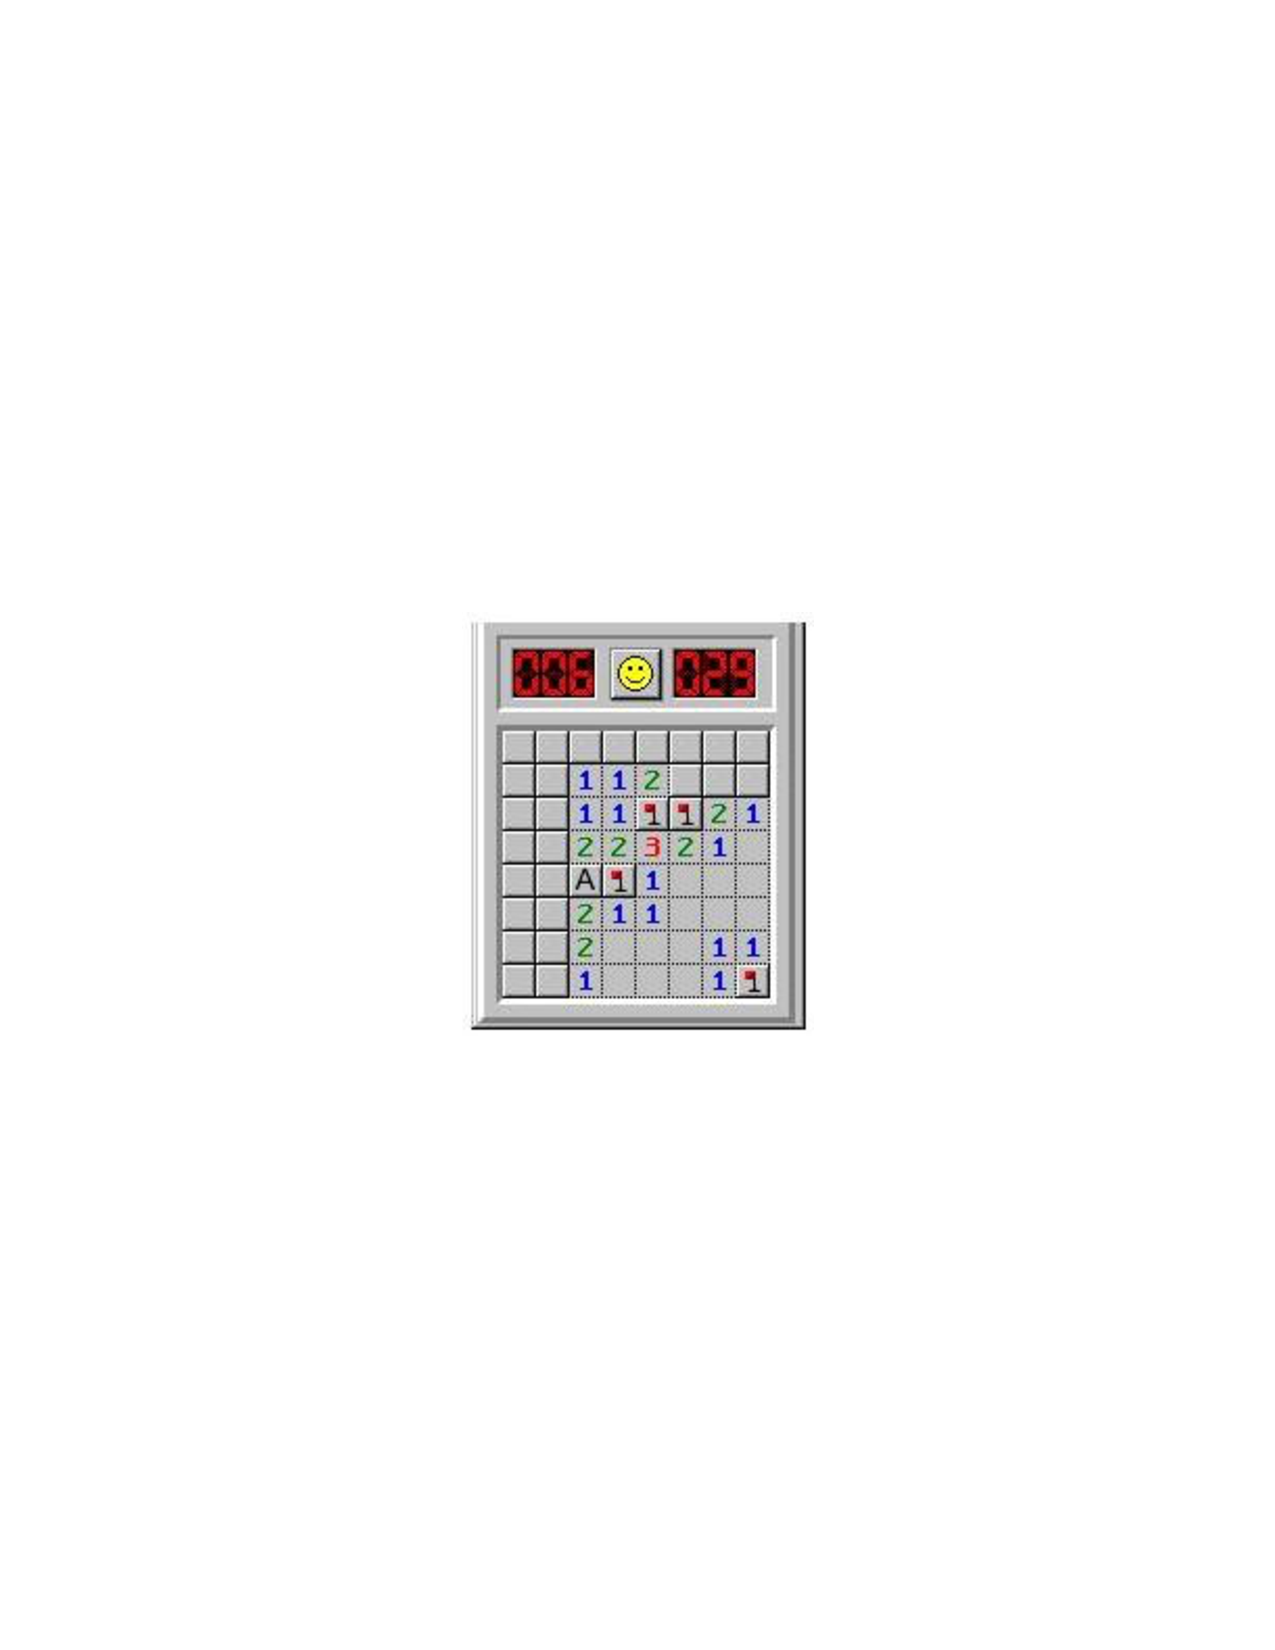
\includegraphics[width=2in]{images/minesweeper1.pdf}

\noindent \textbf{Sample Question:} Determine whether the following statement is true or false and explain. Square A is a mine.

\noindent \textbf{Sample Answer:} FALSE. The square directly below the flag next to the A contains a $1$, indicating that one and only one square adjacent to it is a mine. Since the square above the $1$ (the flag) is a mine, square A must not be a mine. We can conclude that the statement ``Square A is a mine." is false.

%<*truthTables:Minesweeper:entrance:game>
Consider the in-progress game below and determine if each statement below is true or false. Provide a brief justification for your claim.
\par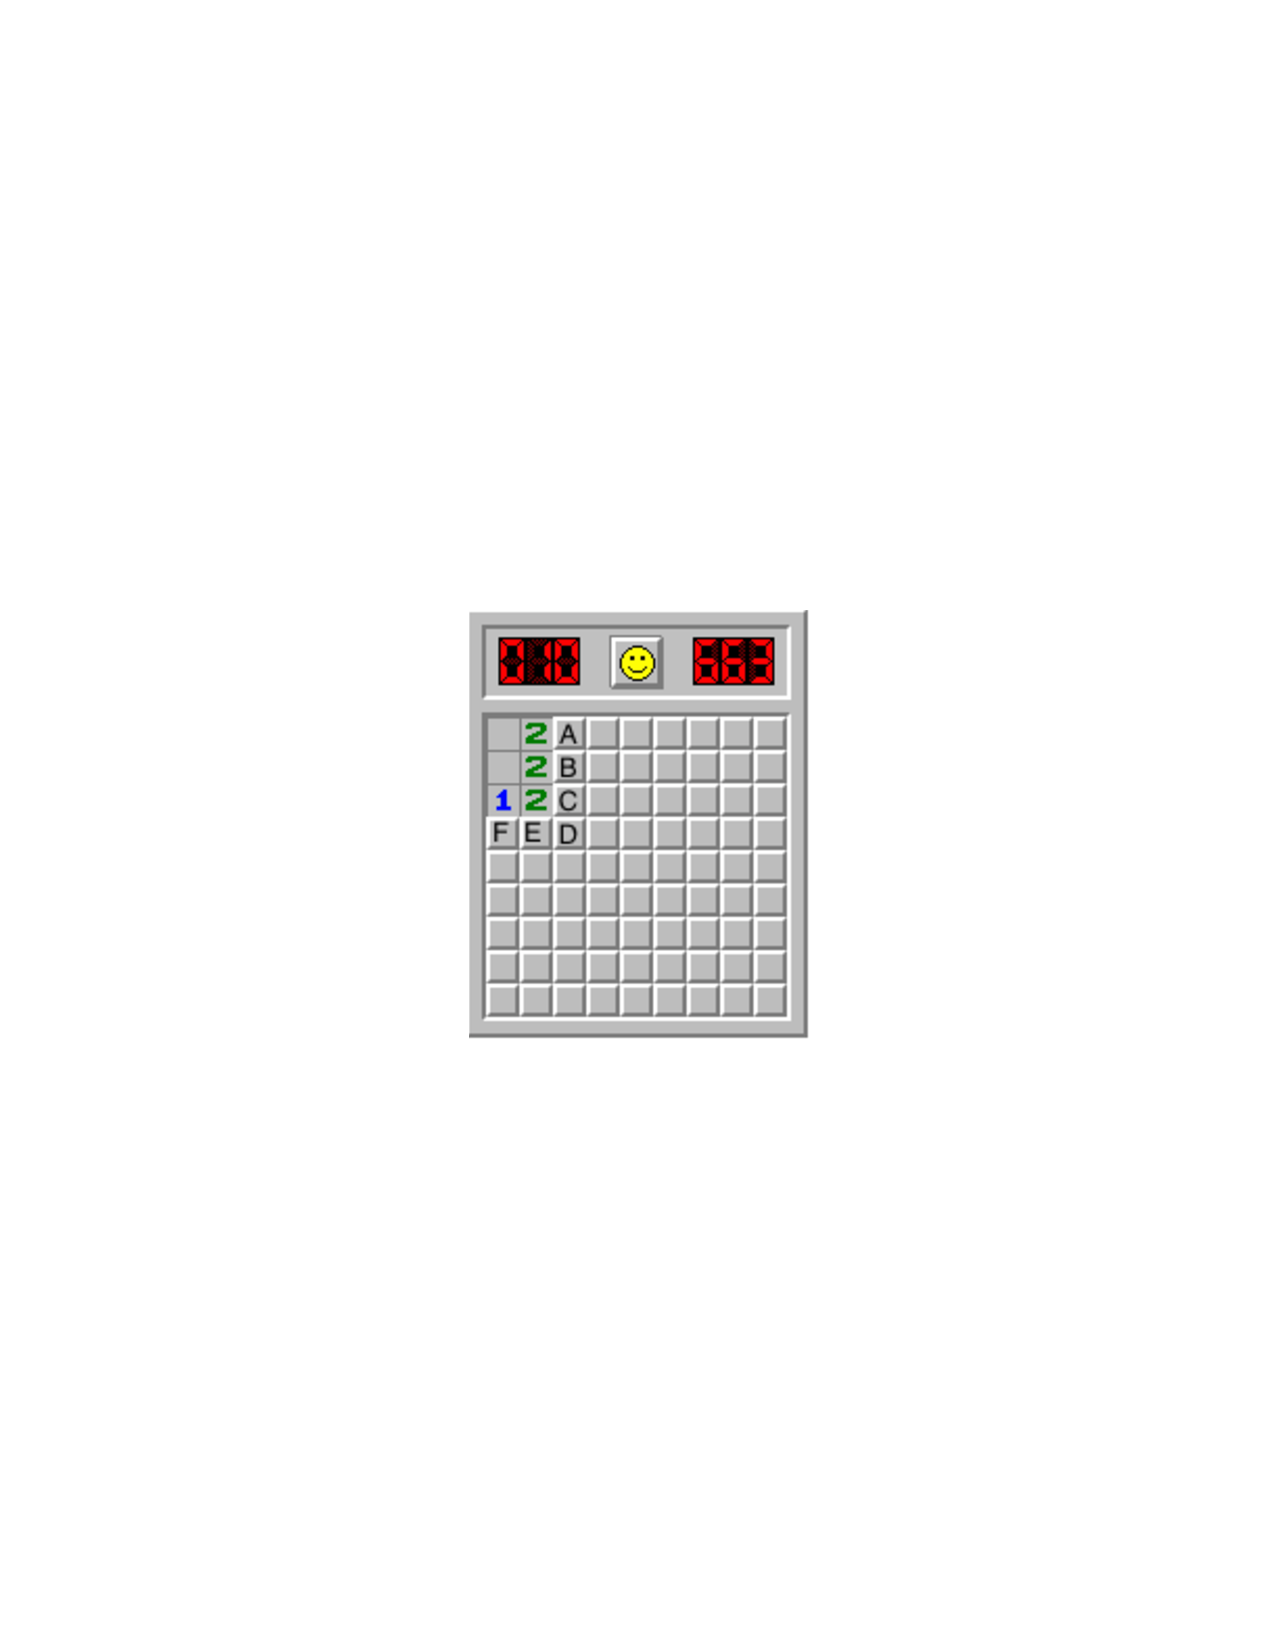
\includegraphics[width=2in]{images/MinesweeperBegin.pdf}
    \begin{enumerate}
        \item Squares A and B are mines.
        \par\Instr{ TRUE. The 2 next to the A requires two adjacent mines, and there are exactly 2 adjacent spaces that have not yet been cleared. Those are squares A and B, so A and B must be the two mines.}
        \wbvfill
        \item Square C is a mine
        \par\Instr{ FALSE. The 2 next to the B requires two adjacent mines. Since squares A and B are mines and are both adjacent, there must be no more mines adjacent to that 2. Since C is adjacent to the 2 also, it cannot be a mine.}
        \wbvfill
        \item Squares F and E are mines
        \par\Instr{ FALSE. There can only be one mine adjacent to the square above F. Since both E and F are adjacent to this square, they cannot both be mines.}
        \wbvfill
        \item Square D is a mine.
        \par\Instr{ FALSE. Squares B,E,F are all adjacent to the 2 above the E. B is a mine and exactly one of E and F is a mine due to the $1$ above the F. Either way, D cannot be a mine since that would place a third mine adjacent to the 2 above the E.}
        \wbvfill
    \end{enumerate}

\newpage
\subsection{Implications in Minesweeper}

In the game Minesweeper sometimes we cannot determine whether a square is a mine or not at first glance. If we can determine the state of a nearby square, however, that may help us figure it out. Here we wish to explore these scenarios and how logic plays a roll in beating the game.

\begin{enumerate}
\item \label{Minesweeper1} Consider this portion of an in-progress game. Are the statements below true, false, or indeterminate (need more information)? Explain.
\par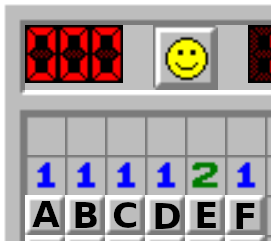
\includegraphics[width=2.5in]{images/MinesweeperImplication01.png}
\begin{enumerate}
    \item A is a mine.
    \par\Instr{ INDETERMINATE. Technically this is a TRUE statement, but it requires a lengthy argument (to be made forthwith). Without looking ahead or going through the investigation, the most likely and appropriate answer is indeterminate.}
    \wbvfill
    \item B is a mine.
    \par\Instr{ INDETERMINATE. Technically this is a FALSE statement, but it requires a lengthy argument (the same one that leads to the conclusion that A is a mine). Without looking ahead or going through the investigation, the most likely and appropriate answer is indeterminate.}
    \wbvfill
    \item \label{Minesweeper1.1} A is a mine or B is a mine.
    \par\Instr{ TRUE. A and B are both adjacent to the leftmost one, so at least one of them must be a mine. Of course the $1$ means exactly one of them must be a mine, but to state that A or B is true is to say that one or the other or both are true (that is, at least one is a mine is all that is needed).}
    \wbvfill
    \item \label{Minesweeper1.2} A is a mine and B is a mine.
    \par\Instr{ FALSE. A and B are both adjacent to the leftmost one, so they cannot both be mines. The combination of this statement being false and the previous statement being true leads to the conclusion (or is the logically equivalent statement) that exactly one of A and B is a mine.}
    \wbvfill
\end{enumerate}
    
\item \label{Minesweeper2} What can we conclude from the exploration in question \ref{Minesweeper1}? Circle one and explain.
\begin{enumerate}
    \item Neither A nor B is a mine.
    \item Both A and B are mines.
    \item Either A is a mine or B is a mine, but not both.
\end{enumerate}
\par\Instr{ From \ref{Minesweeper1.1} and \ref{Minesweeper1.2} (or from the fact that A and B are adjacent to the leftmost $1$), we conclude "Either A is a mine or B is a mine, but not both."}
\wbvfill

\wbnewpage
\item \label{Minesweeper3} So which is it? Is A the mine? or is B? To figure this out logically, we make A a mine and see what happens. So suppose A is a mine (as if we knew this to be a fact) and determine whether the following statements are true or false. You should be able to explain each one. Use the boards below, which show the same board without the letters, for reference.
\begin{enumerate}
    \item If A is a mine, then B is clear.
    \par\Instr{ TRUE. The leftmost $1$ requires exactly one of A and B to be a mine.}
    \wbvfill
    \item If A is a mine, then B is clear and C is clear.
    \par\Instr{ TRUE. C must also be clear because the $1$ above the B is adjacent to both A and C so exactly one of them must be a mine (and we have assumed it is A).}
    \wbvfill
    \item If A is a mine, then B is clear and C is clear and D is a mine.
    \par\Instr{ TRUE. The $1$ above C is adjacent to B,C,D. Since B and C are clear, D must be the mine.}
    \wbvfill
    \item If A is a mine, then B is clear and C is clear and D is a mine and E is a mine and F is a mine.
    \par\Instr{ FALSE. The $1$ above D is adjacent to C,D,E. Since D is a mine, E must not be.}
    \wbvfill
    \item If A is a mine, then B is clear and C is clear and D is a mine and E is a mine and F is clear.
    \par\Instr{ FALSE. The $1$ above D is adjacent to C,D,E. Since D is a mine, E must be clear.}
    \wbvfill
    \item If A is a mine, then B is clear and C is clear and D is a mine and E is clear and F is a mine.
    \par\Instr{ TRUE. The 2 above E is adjacent to D,E,F. Since E is clear, F must be a mine.}
    \wbvfill
    \item If A is a mine, then B is clear and C is clear and D is a mine and E is clear and F is clear.
    \par\Instr{ FALSE. The 2 above E is adjacent to D,E,F. Only one of these squares is clear.}
    \wbvfill
\end{enumerate}
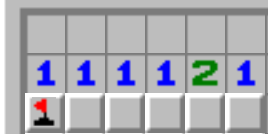
\includegraphics[width=3in]{images/MinesweeperImplication03-A.png} 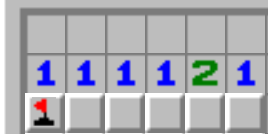
\includegraphics[width=3in]{images/MinesweeperImplication03-A.png}

\wbnewpage
Now suppose B is a mine (as if we knew this to be a fact) and start over, assuming we don't know anything about any other square to begin. Determine whether the following statements are true or false. You should be able to explain each one. Use the boards below, which show the same board without the letters, for reference.
\begin{enumerate} \setcounter{enumii}{7}
    \item If B is a mine, then A is clear.
    \par\Instr{ TRUE. The leftmost $1$ requires exactly one of A and B to be a mine.}
    \wbvfill
    \item If B is a mine, then A is clear and C is clear.
    \par\Instr{ TRUE. C must also be clear because the $1$ above the B is adjacent to both B and C so exactly one of them must be a mine (and we have assumed it is B).}
    \wbvfill
    \item If B is a mine, then A is clear and C is clear and D is clear.
    \par\Instr{ TRUE. The $1$ above C is adjacent to B,C,D. Since B is a mine, D must be clear.}
    \wbvfill
    \item If B is a mine, then A is clear and C is clear and D is clear and E is a mine and F is a mine.
    \par\Instr{ FALSE. The $1$ above the F requires that only one of E and F be a mine.}
    \wbvfill
    \item If B is a mine, then A is clear and C is clear and D is clear and E is a mine and F is clear.
    \par\Instr{ FALSE. The 2 is adjacent to D,E,F. Since D is clear, F cannot also be clear.}
    \wbvfill
    \item If B is a mine, then A is clear and C is clear and D is clear and E is clear and F is a mine.
    \par\Instr{ FALSE. The 2 is adjacent to D,E,F. Since D is clear, E cannot also be clear.}
    \wbvfill
    \par\Instr{ FALSE. The 2 is adjacent to D,E,F. Since D is clear, F cannot also be clear.}
    \wbvfill
\end{enumerate}
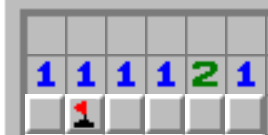
\includegraphics[width=3in]{images/MinesweeperImplication03-B.png} 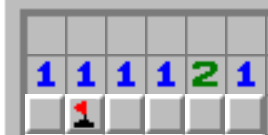
\includegraphics[width=3in]{images/MinesweeperImplication03-B.png}

\wbnewpage
\item \label{Minesweeper4} According to your answers in question \ref{Minesweeper3}, which do you think is the mine? A or B? Explain.
\par\Instr{ By contradiction, B cannot be the mine. There is no way to properly label squares A-F assuming B is a mine. Therefore A must be the mine. Since we have not formally discussed contradiction, however, students may not think this way. They may just have a hunch. Nudge them in the direction of understanding the contradiction, but don't get stuck on this. Let them proceed to the final question where it will be laid out.}
\wbvfill

\item \label{Minesweeper5} Below is more of the board from question \ref{Minesweeper1}. Use this new information to determine whether each square A through J is a mine or is clear. A board without the letters is supplied for you to work on. You may want to use a pencil!
\par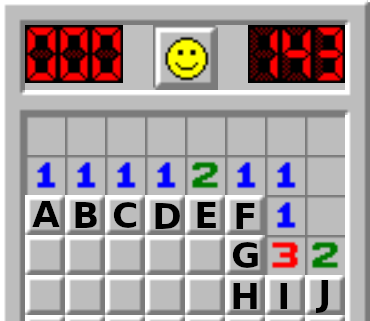
\includegraphics[width=3in]{images/MinesweeperImplication02.png}
\par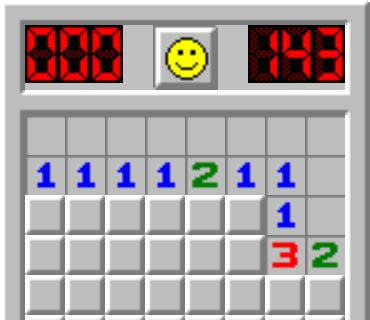
\includegraphics[width=3in]{images/MinesweeperImplication03.png}
\par\Instr{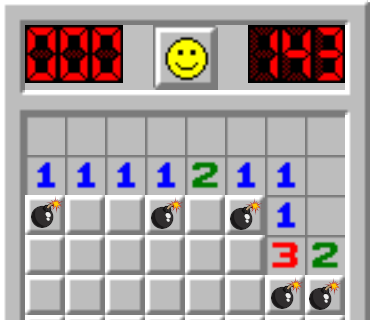
\includegraphics[width=3.25in]{images/MinesweeperImplication03-solved.png}}
\par Were you right about squares A and B?
\wbvfill

\wbnewpage
\item \label{Minesweeper6} Consider the in-progress game below. Are the following statements true or false? Explain.
\par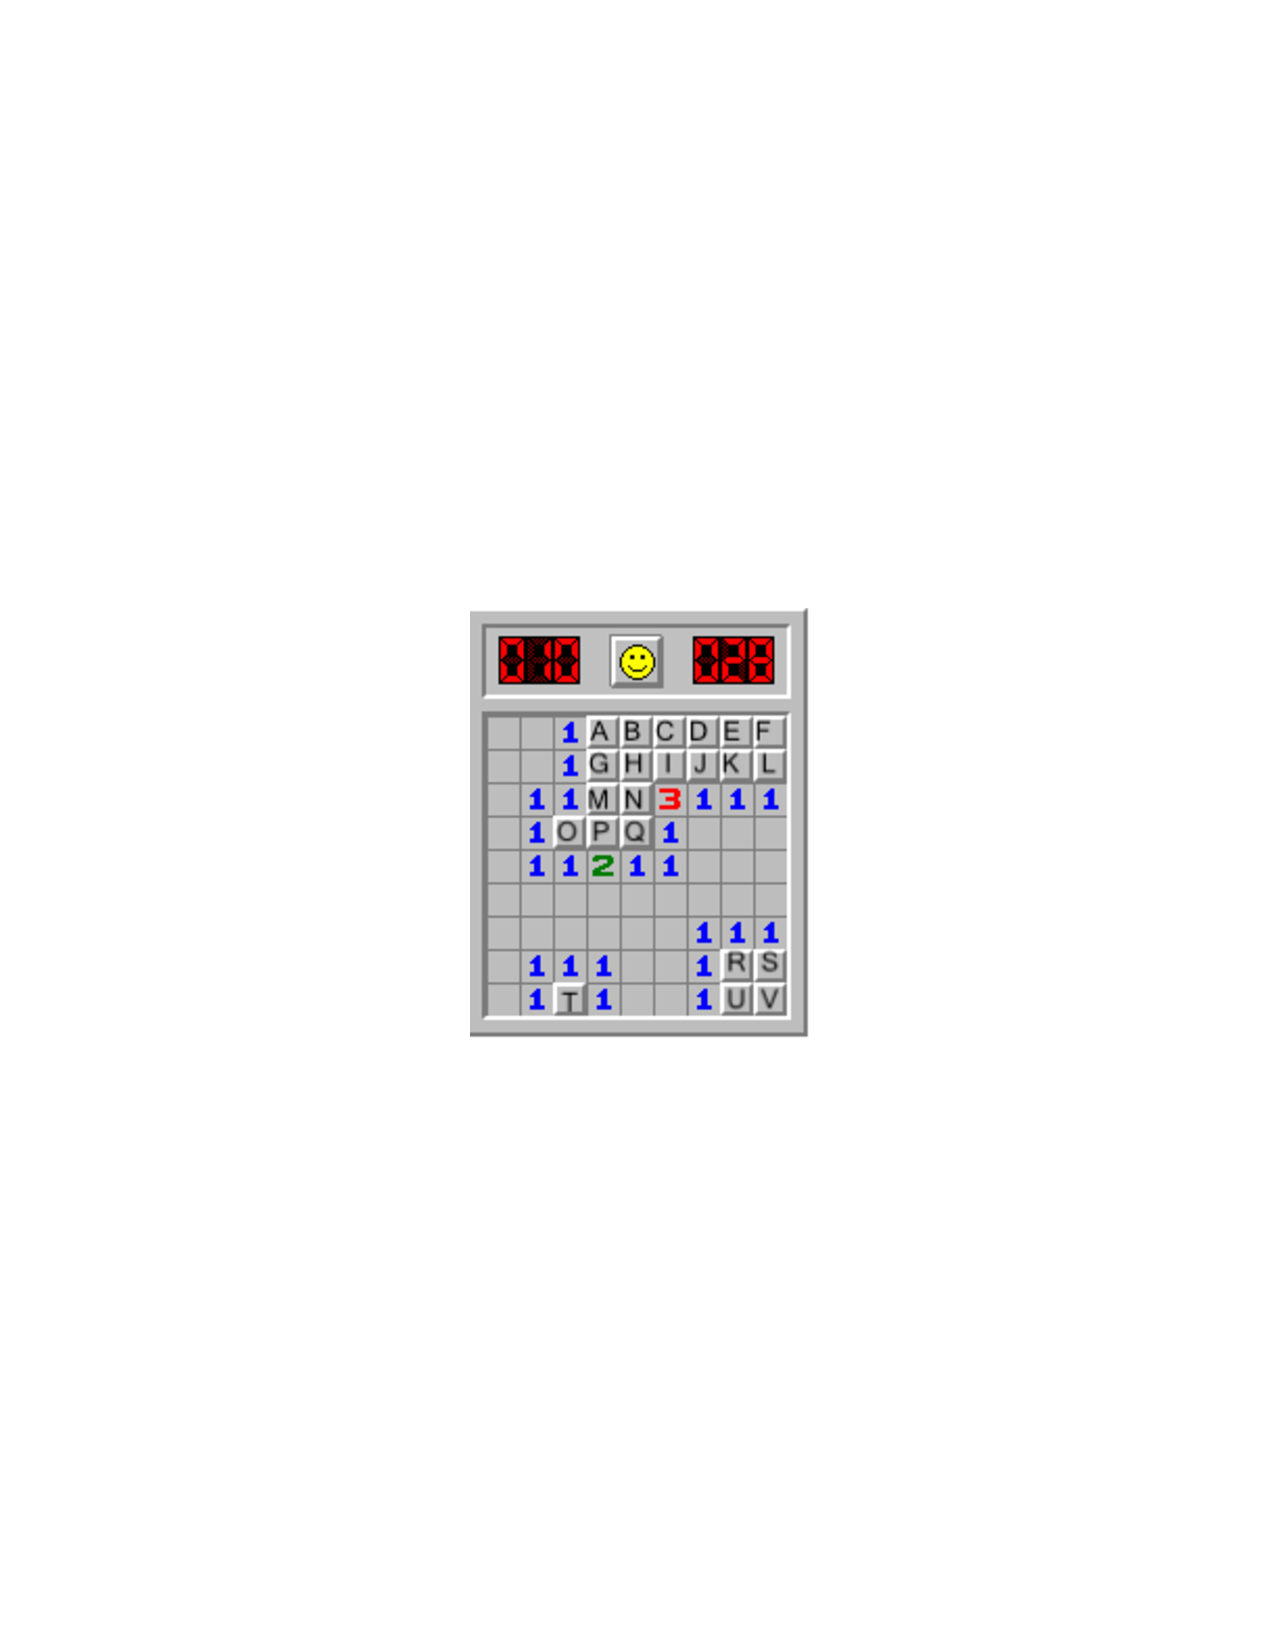
\includegraphics[width=2in]{images/MinesweeperArgument.pdf}
\begin{enumerate}
\item Square Q is a mine.
\par\Instr{ TRUE. The $1$ down and to the right of Q requires an adjacent mine. Since Q is the only uncleared adjacent space it must be the mine.}
\wbvfill
\item Square N is a mine.
\par\Instr{ FALSE. The $1$ next to the Q is, of course, adjacent to the Q. Since Q is a mine, no other space adjacent to the $1$ can be a mine. N is such a space and therefore cannot be a mine.}
\wbvfill
\item Square I is a mine and square J is a mine.
\par\Instr{ FALSE. I and J are both adjacent to the $1$ below J. Therefore they cannot both be mines.}
\wbvfill
\item Square H is a mine.
\par\Instr{ TRUE. The 3 requires three adjacent mines. One of them is at Q. One more is at I or J. N is not a mine. The only other adjacent uncleared square is H, and therefore must be a mine.}
\wbvfill
\item \label{KorL1} Square K is a mine or square L is a mine.
\par\Instr{ TRUE. The $1$ below the L requires it as K and L are the only adjacent uncleared squares.}
\wbvfill
\item \label{KorL2} If square K is a mine, then square J is not a mine.
\par\Instr{ TRUE. J and K are both adjacent to the $1$ under K. Therefore at most one of them can be a mine.}
\wbvfill
\item \label{KorL3} If square L is a mine, then square J is not a mine.
\par\Instr{ TRUE. J and L are both adjacent to the $1$ under K. Therefore at most one of them can be a mine.}
\wbvfill
\item Square J is not a mine.
\par\Instr{ TRUE. Statements \ref{KorL1},\ref{KorL2},\ref{KorL3} prove this. Either K or L is a mine [\ref{KorL1}], and either way J is not a mine [\ref{KorL2},\ref{KorL3}].}
\wbvfill
\end{enumerate}

\wbnewpage
\item Below is an argument table showing that the statement ``Square A is a mine'' is true for the game shown in question \ref{Minesweeper6}.
\begin{table}[htb]
    \centering
    \begin{tabular}{|l|p{3in}|}
        \hline
         True Statement & Reason \\
         \hline
         O is a mine & O is the only uncleared square adjacent to the $1$ on its left.\\
         \hline
         G is not a mine. & G is adjacent to the $1$ above the O (which is a mine).\\
         \hline
         A is a mine or G is a mine, but not both & A and G are the only uncleared squares adjacent to the $1$ next to A.\\
         \hline
         A is a mine. & The second and third rows (of this table) prove A is a mine.\\
         \hline
    \end{tabular}
    \caption{Argument}
    \label{tab:my_label}
\end{table}
Create an argument table for each statement below. You may use the statements in question \ref{Minesweeper6}, and you may bring in new statements as needed.
\begin{enumerate}
    \item Square P is not a mine.
    \wbvfill
	\Instr{ Here is a sample argument table. Students may resist actually writing the table since "it's so easy", but they should be encouraged to write it out for practice, and because what we are really learning here is the exposition of an argument, not just whether they "get it". Can they explain it in clear and concise language? The next exercise is not so easy.
	\begin{table}[htb]
    \centering
    \begin{tabular}{|l|p{3in}|}
        \hline
         True Statement & Reason \\
         \hline
         O is a mine & O is the only uncleared square adjacent to the $1$ on its left.\\
         \hline
         P is not a mine. & P is adjacent to the $1$ below the O (which is a mine).\\
         \hline
    \end{tabular}
    \caption{Sample Argument}
    \label{tab:my_label}
	\end{table}
	}
    \item Square I is a mine.
	\Instr{ Here is a sample argument table. Students are likely to skip writing much of the first several lines since they "are already done", but they should be encouraged to include them for sake of a complete, self-contained argument.
	\begin{table}[htb]
    \centering
    \begin{tabular}{|l|p{3in}|}
        \hline
         True Statement & Reason \\
         \hline
         Q is a mine & O is the only uncleared square adjacent to the $1$ below and to its right.\\
         \hline
         N is not a mine. & Q and N are adjacent to the $1$ next to Q. Since Q is a mine, N is not.\\
         \hline
         K is a mine or L is a mine & K and L are the only uncleared squares adjacent to the $1$ below L.\\
         \hline
         If K is a mine, then J is not a mine & J and K are both adjacent to the $1$ under K.\\
         \hline
         If L is a mine, then J is not a mine & J and L are both adjacent to the $1$ under K.\\
         \hline
         J is not a mine & The previous three lines in this table prove J is not a mine.\\
         \hline
         I is a mine & There are 5 uncleared squares adjacent to the 3: Q,N,H,I, and J. Since N and J are not mines, the other three must be, including I.\\
         \hline
    \end{tabular}
    \caption{Sample Argument}
    \label{tab:my_label}
	\end{table}
	}
    \wbvfill
\end{enumerate}
\end{enumerate}
\newpage


\subsection{Exit Slip}

For the in-progress game below, create three true statements, one for each type listed below.

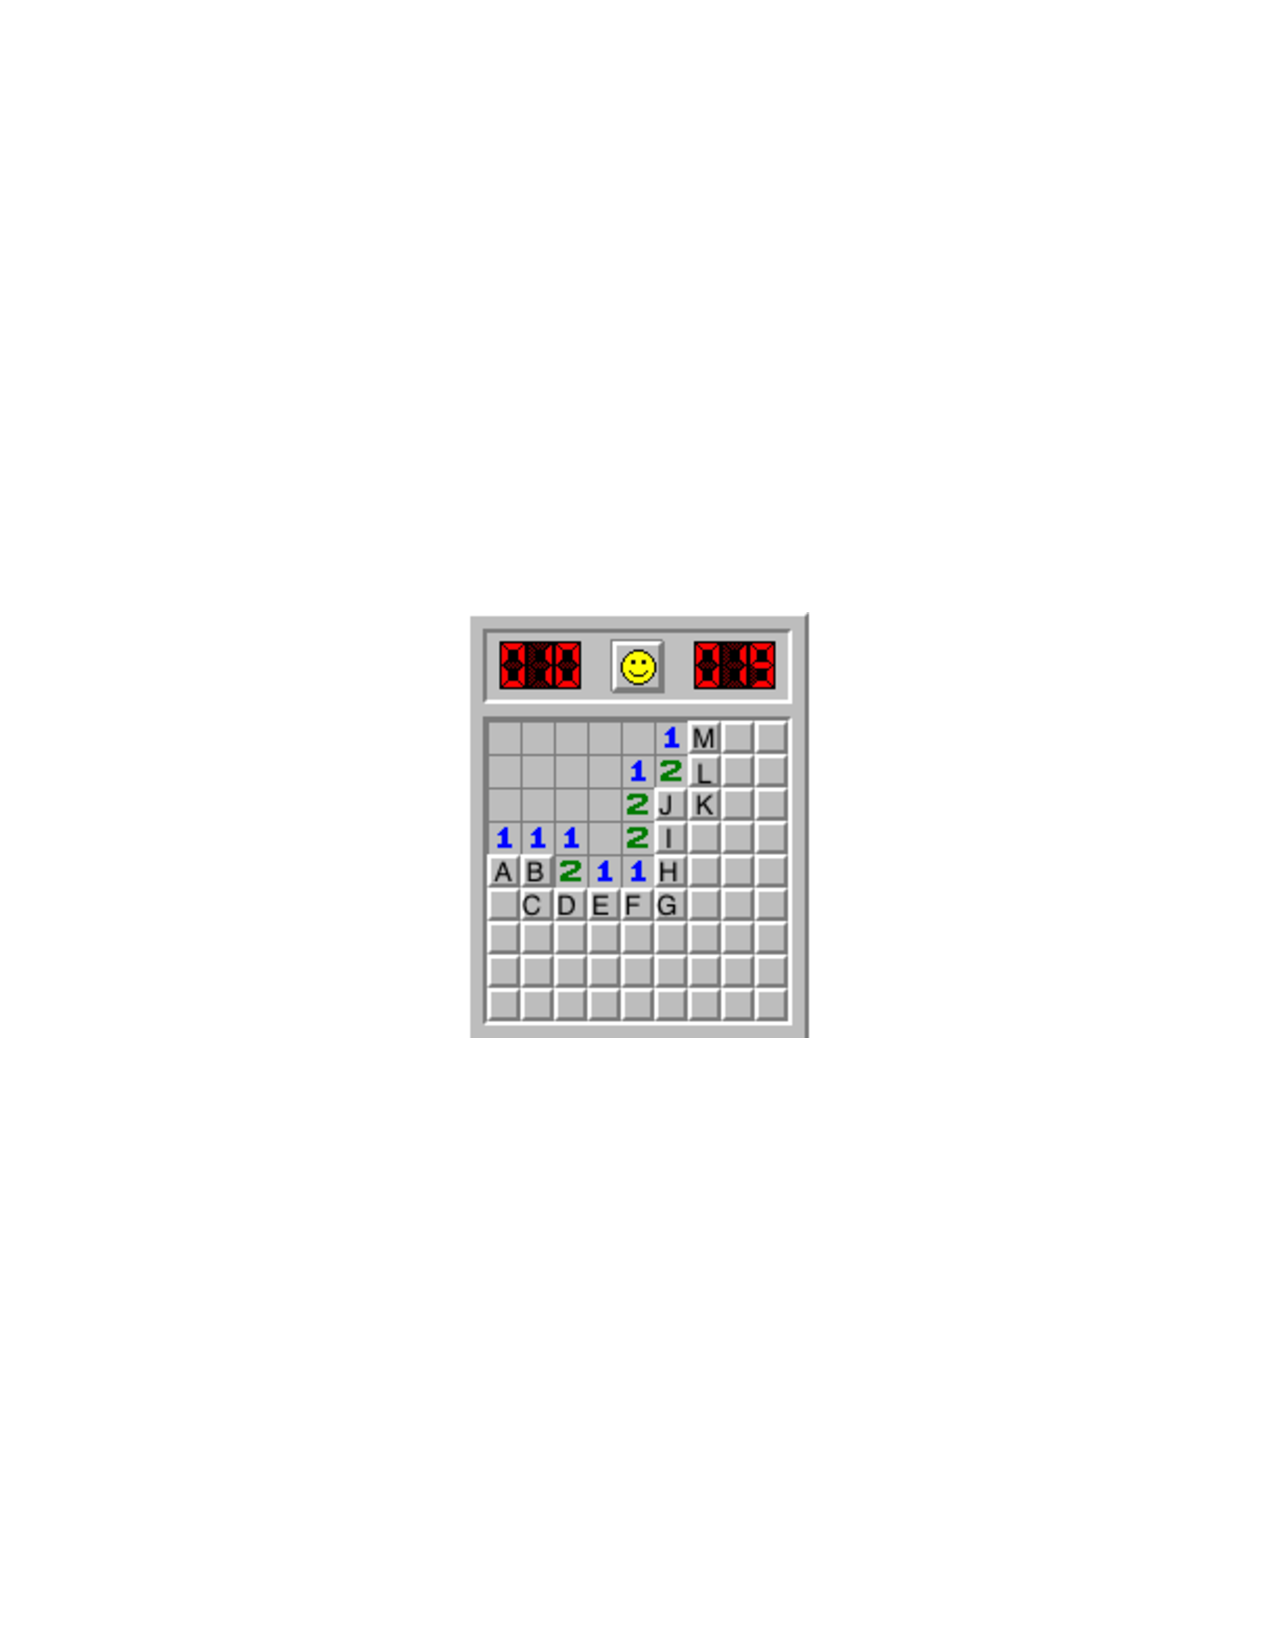
\includegraphics[width=3in]{images/MinesweeperExit.pdf}

\begin{enumerate}
    \item Statement containing an ``and''
    
    \item Statement containing an ``or''
    
    \item An implication statement in the form `` If \dots, then \dots.''
\end{enumerate}
\wbnewpage


\iffalse
%<*truthTables:statement:negation:intro>
\subsection{Activity: Negation}\label{negation}
%</truthTables:statement:negation:intro>

\Instr{  
Goals for this activity:
\begin{packedItem}
\item Working with negations withing compound statements; 
\item Determining truth values of compound statements containing negations; 
\item Completing Truth Tables for compounstatements containing negations; and
\item Determining weather two statements are equivalent.
\end{packedItem}
}

%<*truthTables:statement:negation:intro2>
\indent Let $\neg P$ represent the statement\index{statement} ``$P$ is false''. ($\neg P$\index{$\neg$} is called the negation of $P$.) Again we will consider the statements below.
\begin{center}
\begin{tabular}{ll}
$P$: & I am wearing a top hat.\\
$Q$: & I am wearing overalls.\\
$R$: & I am wearing rain boots.\\
\end{tabular}
\end{center}

\begin{enumerate}
\setcounter{enumi}{26}
\item\label{negPtrue} If $\neg P$ is true, is anything on my head? 
%</truthTables:statement:negation:intro2>

\Instr{  When $\neg P$ is true, ``$P$ is false'' is true, so I am not wearing a top hat. So there maybe something on my head, but it is not a top hat!}

%<*truthTables:statement:negation:negPtrue>
\item If $\neg P$ is false, is anything on my head?
%</truthTables:statement:negation:negPtrue>

\Instr{  When $\neg P$ is false, ``$P$ is false'' is false, so $P$ is true. Therefore there is something on my head when $\neg P$ is false, namely a top hat.}

%<*truthTables:statement:negation:negPfalse>
\item Fill in the truth table\index{truth table} below. Each cell in the table should contain either ``True'' or ``False.'' As in Question~{\normalfont\ref{logicTable}} begin by completing the first column.
\begin{center}
\begin{tabular}{|c||c|}
\hline
$P$ & $\neg P$ \\
\hline
\hline
\hspace{.75in} & \hspace{.75in} \\
\hline
& \\
\hline
\end{tabular}
\end{center}
%</truthTables:statement:negation:negPfalse>

\Instr{  
\begin{center}
\begin{tabular}{|c||c|}
\hline
$P$ & $\neg P$ \\
\hline
\hline
True & False \\
\hline
False & True \\
\hline
\end{tabular}
\end{center}
}

%<*truthTables:statement:negation:PwedgeRfalse>
\item Suppose you know the statement $P\wedge R$\index{$\wedge$} is false. Describe what I'm wearing. Is there a statement that says the same thing when it is true?
%</truthTables:statement:negation:PwedgeRfalse>

\Instr{  If $P\wedge R$ is false then it is not the case that I am wearing both a top hat and rain boots. Therefore I am either ``not wearing a top hat'' or ``I am not wearing rain boots.'' The easiest way to find a corresponding true statement is to simply apply the $\neg$ function and use $\neg (P\wedge R)$. But the verbal description of what I'm wearing leads to another solution: $\neg P \vee \neg Q$\index{$\neg$}\index{$\vee$}. Encourage the students to find both answers.}

%<*truthTables:statement:negation:QveeRfalse>
\item Suppose you know the statement $Q\vee R$ is false. Describe what I'm wearing. Is there a statement\index{statement} that says the same thing when it is true?
%</truthTables:statement:negation:QveeRfalse>

\Instr{  If $Q\vee R$ is false then it is not the case that either I am wearing overalls or I am wearing rain boots. So I cannot be wearing either. Therefore I am not wearing overalls and I am not wearing rain boots. So both the statement\index{statement} $\neg Q \wedge \neg R$\index{$\neg$}\index{$\wedge$} is true. What I am wearing is also described by $\neg(Q\wedge R)$, as can be seen by applying the definition of $\neg$. So both are good answers.}

%<*truthTables:statement:negation:PwedgenegQfalse>
\item Suppose you know that statement $P\wedge \neg Q$ is false. Describe what I'm wearing. Is there a statement that says the same thing when it is true?
%</truthTables:statement:negation:PwedgenegQfalse>

\Instr{  If $P\wedge \neg Q$ is false then it is not the case that I am both wearing a top hat and not wearing overalls. Therefore either I am not wearing a top hat or I am wearing overalls. So the statement\index{statement} $\neg P\vee Q$\index{$\neg$}\index{$\vee$}\index{$\wedge$} is true. Also, $\neg(P\wedge \neg Q)$ is true by the definition of $\neg$. So both are good answers.}

%<*truthTables:statement:negation:logicTable2.5>
\item\label{logicTable2.5} Fill in the truth table\index{truth table} below so that each cell contains either ``True'' or ``False.'' As in Question~{\normalfont\ref{logicTable}}, begin by completing the first two columns so that all ways truth values can be assigned to $P$ and $Q$ are represented in the four rows.
\begin{center}
\begin{tabular}{|c|c||c|c|c|c|}
\hline
$P$ & $Q$ & $\neg P$ & $\neg Q$ & $\neg(P\wedge Q)$ & $\neg P\vee \neg Q$ \\
\hline
\hline
\hspace{.5in} & \hspace{.5in} & \hspace{.5in} & \hspace{.5in} & \hspace{.75in} & \hspace{.75in} \\
\hline
&&&&& \\
\hline
&&&&& \\
\hline
&&&&& \\
\hline
\end{tabular}
\end{center}
%</truthTables:statement:negation:logicTable2.5>

\Instr{ 
\begin{center}
\begin{tabular}{|c|c||c|c|c|c|}
\hline
$P$ & $Q$ & $\neg P$ & $\neg Q$ & $\neg (P\wedge Q)$ & $\neg P\vee \neg Q$ \\
\hline
\hline
True & True & False & False & False & False  \\
\hline
True & False & False & True & True & True  \\
\hline
False & True & True & False & True & True \\
\hline
False & False & True & True & True & True \\
\hline
\end{tabular}
\end{center}
}

%<*truthTables:statement:negation:sameStatement?>
\item Using the truth table\index{truth table} in Question~{\normalfont\ref{logicTable2.5}} determine if the statement $\neg(P\wedge R)$ is the same as the statement\index{statement}\index{$\wedge$}\index{$\vee$}\index{$\neg$} $\neg P \vee \neg R$. Explain yourself thoroughly.
%</truthTables:statement:negation:sameStatement?>

\Instr{  Based on the truth table they are the same. Also, by reasoning out what each of the statements is saying, it is clear that the two statements are identical.}

%<*truthTables:statement:negation:logicTable3>
\item\label{logicTable3} Fill in the table below so that each cell contains either ``True'' or ``False.'' As in Question~{\normalfont\ref{logicTable}}, begin by completing the first two columns.
\begin{center}
\begin{tabular}{|c|c||c|c|c|c|c|}
\hline
$P$ & $Q$ & $\neg P$ & $\neg Q$ & $\neg P\wedge Q$ & $P\vee \neg Q$ & $\neg P\vee \neg Q$ \\
\hline
\hline
\hspace{.5in} & \hspace{.5in} & \hspace{.5in} & \hspace{.5in} & \hspace{.75in} & \hspace{.75in} & \hspace{.75in} \\
\hline
&&&&&& \\
\hline
&&&&&& \\
\hline
&&&&&& \\
\hline
\end{tabular}
\end{center}
%</truthTables:statement:negation:logicTable3>

\Instr{  
\begin{center}
\begin{tabular}{|c|c||c|c|c|c|c|}
\hline
$P$ & $Q$ & $\neg P$ & $\neg Q$ & $\neg P\wedge Q$ & $\neg P\vee \neg Q$ & $P\vee \neg Q$ \\
\hline
\hline
True & True & False & False & False & False & True \\
\hline
True & False & False & True & False & True & True \\
\hline
False & True & True & False & True & True & False \\
\hline
False & False & True & True & False & True & True \\
\hline
\end{tabular}
\end{center}
}

%<*truthTables:statement:negation:logicTable4>
\item\label{logicTable4} Fill in the table below so that each cell contains either ``True'' and ``False.'' As in Question~{\normalfont\ref{logicTable}}, begin by completing the first three columns.
\begin{center}
\begin{tabular}{|c|c|c||c|c|c|}
\hline
$P$ & $Q$ & $R$ & $(P\wedge Q) \wedge \neg R$ & $(\neg P \vee \neg Q) \vee R$ & $(P\vee \neg Q) \wedge \neg R$ \\
\hline
\hline
\hspace{.5in} & \hspace{.5in} & \hspace{.5in} &&& \\
\hline
&&&&& \\
\hline
&&&&& \\
\hline
&&&&& \\
\hline
&&&&& \\
\hline
&&&&& \\
\hline
&&&&& \\
\hline
&&&&& \\
\hline
\end{tabular}
\end{center}
%</truthTables:statement:negation:logicTable4>

\Instr{  
\begin{center}
\begin{tabular}{|c|c|c||c|c|c|}
\hline
$P$ & $Q$ & $R$ & $(P\wedge Q) \wedge \neg R$ & $(\neg P \vee \neg Q) \vee R$ & $(P\vee \neg Q) \wedge \neg R$ \\
\hline
\hline
True & True & True & False & True & False \\
\hline
True & True & False & True & False & True \\
\hline
True & False & True & False & True & False \\
\hline
True & False & False & False & True & True \\
\hline
False & True & True & False & True & False \\
\hline
False & True & False & False & True & False \\
\hline
False & False & True & False & True & False \\
\hline
False & False & False & False & True & True \\
\hline
\end{tabular}
\end{center}
}

%<*truthTables:statement:negation:negnegP>
\item Write out what it means if the statement\index{statement} $\neg (\neg P))$\index{$\neg$} is true.
%</truthTables:statement:negation:negnegP>

\Instr{  The statement $\neg(\neg P))$ means it is not the case that I am not wearing a top hat. In other words, I am wearing a top hat; so $P$ is true.}

%<*truthTables:statement:negation:end>
\end{enumerate}
%</truthTables:statement:negation:end>
\fi

%<*truthTables:conditional:title>
\section{Extension Activity: Arguments}

\subsection{Activity: Nancy Out On The Town}\label{conditional}
%</truthTables:conditional:title>

\Instr{  
Goals for this activity:
\begin{packedItem}
\item Discovering the implications of compound statements containing dependant statements; 
\end{packedItem}
}

%<*truthTables:conditional:intro>
\indent Nancy's friends are trying to find her based on whether the following statements\index{statement} are true or false. They know that she is at exactly one of: home, the movie theater, the grocery store, or a clothing store.
\begin{center}
\begin{tabular}{ll}
$P$: & Nancy is at home. \\
$Q$: & Nancy is at the movie theater. \\
$R$: & Nancy is at the grocery store. \\
$S$: & Nancy is at a clothing store. \\
$T$: & Nancy is trying on clothes. \\
$U$: & Nancy is buying food.
\end{tabular}
\end{center}

\begin{enumerate}
\item If $P$ is true is $Q$ true or false? Explain your reasoning.
%</truthTables:conditional:intro>

\Instr{  It is clear that someone can't be in two places at once. So your home cannot be at the movie theater and statement $Q$ is false.}\wbvfill

%<*truthTables:conditional:IfQthenP>
\item What statements could be true if $T$ is true? Explain your reasoning.
%</truthTables:conditional:IfQthenP>

\Instr{  If $T$ is true, then we must identify the locations where Nancy could possibly be. Those locations would be home or the clothing store. So one of $P$ and $S$ could be true.}\wbvfill

%<*truthTables:conditional:IfPthenQorR>
\item If $P$ is true, is $T\vee U$\index{$\vee$} true or false? Explain your answer.
%</truthTables:conditional:IfPthenQorR>

\Instr{  If $P$ is true, then Nancy is at home. She cannot buy food at home (unless she does so over the internet!), but she can be trying on clothes at home. Since we are using the ``or'' operator, the statement $T\vee U$ could be true, but may be false if at the moment she is doing other things like cooking dinner.
}\wbvfill

%<*truthTables:conditional:IfPthenNotS>
\item If $P$ is true, is $\neg S$\index{$\neg$} true or false? Explain your answer.
%</truthTables:conditional:IfPthenNotS>

\Instr{  Notice that $\neg S$ means that Nancy is not at the clothing store. Since she is at home, $\neg S$ is true in this case.}\wbvfill

%<*truthTables:conditional:IfQorRthenP>
\item What statements are false if $Q\vee R$ is true? 
%</truthTables:conditional:IfQorRthenP>

\Instr{  The statement $Q\vee R$ is true states that Nancy is at the movie theater or at the grocery store. So she cannot be at home, nor is she at the clothing store. She is also not trying on clothes. So $P$,  $S$, and $T$ are false.}\wbvfill

%<*truthTables:conditional:IfUthenQandR>
\item If $U$ is true, is $Q\wedge R$\index{$\wedge$} true or false? Explain your conclusion.
%</truthTables:conditional:IfUthenQandR>

\Instr{  If $U$ is true, then Nancy is buying food. It is possible to buy food at both the grocery store and the movie theater. So $Q\wedge R$ is true.} \wbvfill

%<*truthTables:conditional:IfPthenTrue>
\item If $U$ is false, what do you know must be false? Explain your answer.
%</truthTables:conditional:IfPthenTrue>

\Instr{  If Nancy is not buying food, then she cannot be at the grocery store. So $R$ is false. Students may find another reason to be at the grocery store--if you consider it a good reason then there are no statements\index{statement} that you know are definitely false.}\wbvfill

%<*truthTables:conditional:IfPtrueQfalse>
\item If $T$ is true and $U$ is false, what single true statement can you create concerning Nancy's location? Explain your results.
%</truthTables:conditional:IfPtrueQfalse>

\Instr{  If Nancy is trying on clothes and not buying food, then Nancy is either at home or at the clothing store. So the statement $P\vee S$\index{$\vee$} is true.}\wbvfill

%<*truthTables:conditional:QRST>
\item If $U$ is true, what single true statement can you create concerning Nancy's locations? Explain your results.
%</truthTables:conditional:QRST>

\Instr{  Since Nancy is buying food, Nancy is either at the movie theater or at the grocery store. So $Q\vee R$\index{$\vee$} is true. Some students may raise the issue of buying food on the internet making $P$ another possible answer. This is fine as long as the students explain themselves, in which case the answer would be $P\vee Q\vee R$.}\wbvfill

%<*truthTables:conditional:IfTtrue>
\item If $P$ is true and $Q$ is false, is $R\vee(T\wedge U)$\index{$\wedge$} true or false? Explain your results.
%</truthTables:conditional:IfTtrue>

\Instr{  Since Nancy is at home, Nancy is not at the grocery store (so $R$ is false) and cannot be buying food at her home (so $U$ is false), so $R\vee(T\wedge U)$ must be false. Even if students want to allow the possibility of buying food at home on the internet, it would be difficult (impossible?) to do so while trying on clothes, so $T\wedge U$ is false; so even in this case $R\vee(T\wedge U)$ is false.}\wbvfill

%<*truthTables:conditional:IfnegTtrue>
\item If $T$ is true, is $\neg Q \wedge(S\vee P)$\index{$\neg$} true or false? Why?
%</truthTables:conditional:IfnegTtrue>

\Instr{  Since Nancy is trying on clothes, she cannot be at the movie theater (so $\neg Q$ is true), nor is she at the grocery store. So she must be at home or the clothing store. So $\neg Q\wedge (S\vee P)$ is true.} \wbvfill
%<*truthTables:conditional:end>
\end{enumerate}
%</truthTables:conditional:end>

%<*truthTables:implications:title>


\wbnewpage

\section{Project Choices}
\Instr{ Students should complete one of the following projects.}
\begin{enumerate}
    \item \textbf{Project Question:} You are given an in-progress Minesweeper game. On the given board:
    \begin{enumerate}
        \item Mark each box adjacent to a numbered square with an O if it can be determined to be a mine or X if it can be determined that it is not a mine.
        \textit{* There are at least 3 squares that are mines and at least 3 squares that are not mines. There may also be squares adjacent to the numbers that cannot be determined. Leave them blank. *}
        \item Write an argument table for one of the squares marked with an O. \textit{* Do not pick a square located in a ``corner'' adjacent to a square with a $1$. *}
        \item Write an argument table for one of the squares marked with an X.
    \end{enumerate}

    You may want to visit \href{https://freeminesweeper.org/}{https://freeminesweeper.org/} to learn or practice the game.
    
    \item \textbf{Project Question:} You are given an empty nonogram board. Your project is to do the following.
    \begin{enumerate}
        \item Fill all squares correctly, making note of your logic.
        \item Write one true (compound) logical statement that includes an ``and'' and helped you complete the puzzle.
        \item Write one true (compound) logical statement that includes an ``or'' and helped you complete the puzzle.
    \end{enumerate}
    The rules for filling the board are as follows.
    \begin{itemize}
        \item Each box must be filled in black or marked with X.
        \item Beside each row of the grid are listed the lengths of the runs of consecutive black squares on that row.
        \item Above each column are listed the lengths of the runs of consecutive black squares in that column. 
        \item Boxes that are not part of a run of black squares must be marked with X.
    \end{itemize}
    \wbnewpage
    Here is an example of a puzzle in progress.
    \begin{center}
        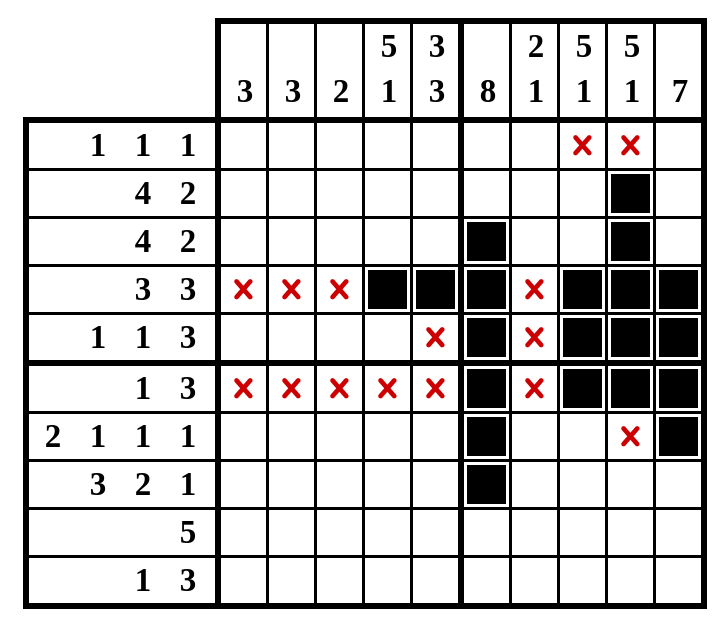
\includegraphics[width=5in]{images/nonogram00.png}
    \end{center}
    The four squares in the rightmost column were filled in first. 7 consecutive squares in that column must be filled in and there are only 10 squares total, so you can only skip three of them from the top \textbf{or} three of them from the bottom. The black squares and X's immediately to the left of those four were filled in next. For example, in row 4 the tenth square in that row is filled in \textbf{and} the last run of squares must be length 3, so the two squares next to the last one must also be filled in black. That completes the run so the square next to that (the 6th from the left in that row) must not be filled (so is marked with an X). See if you can figure out why the rest of the marked squares are the way they are.

    You may want to visit \href{https://www.puzzle-nonograms.com/}{https://www.puzzle-nonograms.com/} to try some nonogram puzzles at a variety of difficulty levels online.

    \item \textbf{Project Question:} You are given two KenKen puzzles. Your project is to do the following.
    \begin{enumerate}
        \item Fill all squares correctly in each puzzle, making note of your logic.
        \item Write one true (compound) logical statement that includes an ``and'' and helped you complete the puzzle.
        \item Write one true (compound) logical statement that includes an ``or'' and helped you complete the puzzle.
    \end{enumerate}
    The rules for solving a KenKen are as follows.
    \begin{itemize}
        \item The only numbers you may write are $1,2,3,\ldots$ up to the number of rows and columns. In a $4\times4$ puzzle you will use the numbers 1 through 4. In a $6\times6$ puzzle you will use the numbers 1 through 6, and so on.
		\item Every allowable number must appear in every row and every column. No number may be repeated in any row or any column.
		\item Each region bounded by a heavy border, called a \textbf{cage}, contains a target number and usually an arithmetic operation. You must fill that cage with numbers that reach the target using the specified arithmetic operation. Numbers may repeat within a cage, if needed, as long as they do not repeat within a single row or column.
    \end{itemize}
    Here is an example of a puzzle in progress.
    \begin{center}
        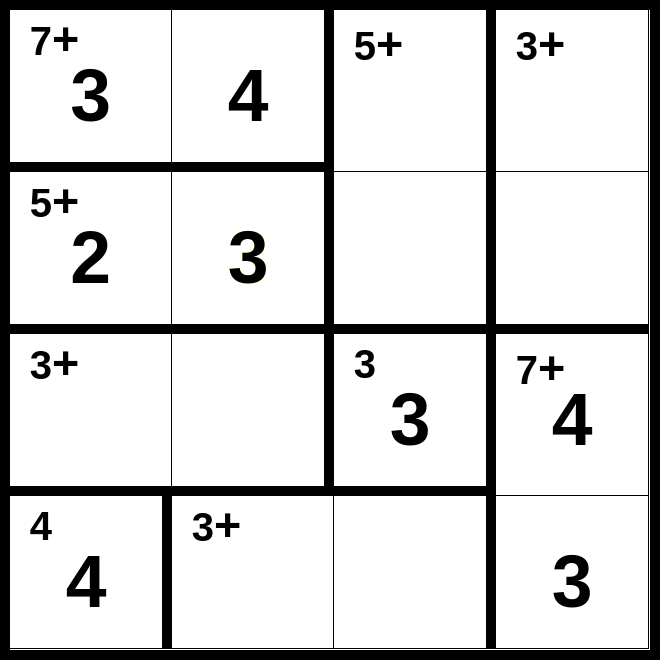
\includegraphics[width=2.5in]{images/kenken00.png}
    \end{center}
    Here is how the numbers were filled in to this point.

    \begin{tabular}{p{3.5in}p{2in}}
         \begin{itemize}\item The $4$ in the bottom left corner and the $3$ in the third row, third column were filled in first. Their cages are only one block so there is no operation to consider. The target number is the number that needs to be filled in.\end{itemize} & \raisebox{-2in}{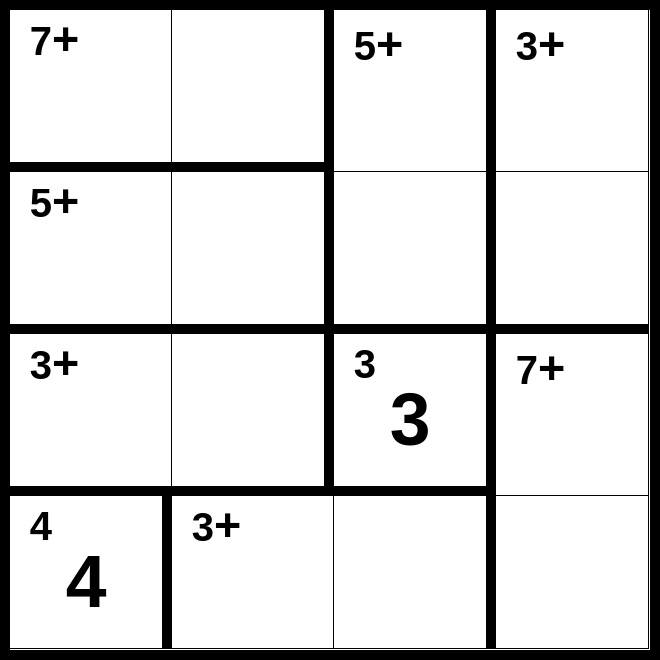
\includegraphics[width=1.9in]{images/kenken00-2.png}}\\
    \end{tabular}
    \begin{tabular}{p{3.5in}p{2in}}
         \begin{itemize}\item The two cages with $7+$ in them were filled in next. In each cage, the numbers $3$ and $4$ must be placed since the only way for two \textbf{different} numbers between 1 and 4 to add up to seven is to use $3$ and $4$. For the cage in the bottom right, the $4$ must be in the third row since there is already a $3$ in that row. You can come to the same conclusion by noticing there is a $4$ in the fourth row (bottom left corner) already, so the $4$ for this cage cannot be put in the fourth row. See if you can understand why the $3$ and $4$ in the $7+$ cage in the top left of the board were placed the way they were. They cannot be placed the other way around.\end{itemize} & \raisebox{-2in}{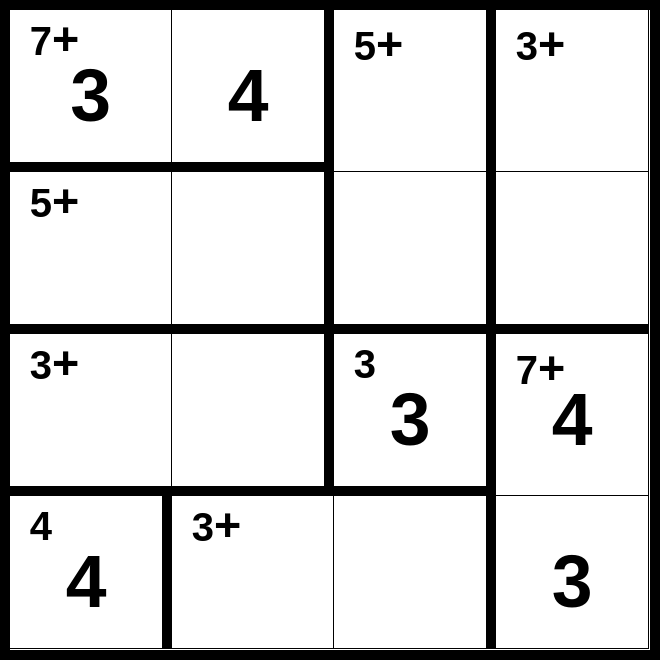
\includegraphics[width=1.9in]{images/kenken00-3.png}}\\
    \end{tabular}
    \begin{tabular}{p{3.5in}p{2in}}
         \begin{itemize}\item The $5+$ cage with the $2$ and $3$ in it was filled in next. There are two ways to use different numbers between 1 and 4 to sum to five---$1$ and $4$ or $2$ and $3$. However, there are already $4$'s in columns one and two, so a $4$ cannot be used in this cage. Hence the cage will be filled with $2$ and $3$. Since there is already a $3$ in column one, the $3$ for this cage must be in column two and therefore the $2$ must be in column one.\end{itemize} & \raisebox{-2in}{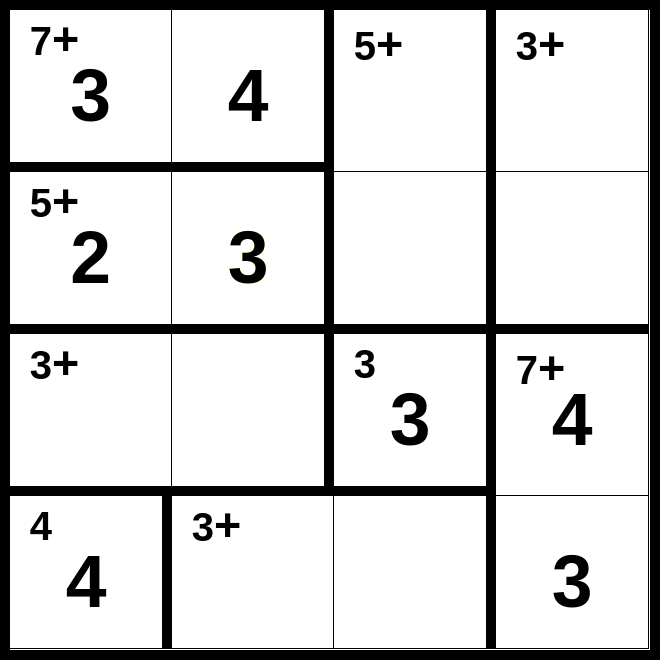
\includegraphics[width=1.9in]{images/kenken00.png}}\\
    \end{tabular}

    See if you can complete the puzzle. HINT: The first column already has the numbers $2,3,4$ in it. There is only one number that can be put in the empty box of that column!

    You may want to visit \href{https://www.kenkenpuzzle.com/}{https://www.kenkenpuzzle.com/} to try some KenKen puzzles at a variety of difficulty levels online. Begin by clicking the "Create Custom Puzzle" button.

    \item \textbf{Project Question:} You are given a Sudoku Pair Puzzle. This isn't your regular Sudoku though! Your project is to do the following.
    \begin{enumerate}
        \item Fill all squares correctly in each puzzle, making note of your logic.
        \item Write one true (compound) logical statement that includes an ``and'' and helped you complete the puzzle.
        \item Write one true (compound) logical statement that includes an ``or'' and helped you complete the puzzle.
    \end{enumerate}

	\textbf{(2,3) - Sudoku Pair Puzzle Rules}: Each completed puzzle is a 6 by 6 grid that contains exactly one integer from 1 to 6 in each cell. Furthermore, there are regions that must contain every integer exactly once. The regions are described below and outlined in the puzzle:
	\begin{enumerate}
		\item Each row is its own region.
		\item Each column is its own region.
		\item Each 2 by 3 rectangle outlined by bold lines is its own region.
		\item Each 3 by 2 rectangle outlined by dashed lines is its own region.
	\end{enumerate}
	\begin{center}
		Here is an example of a completed puzzle.\par
		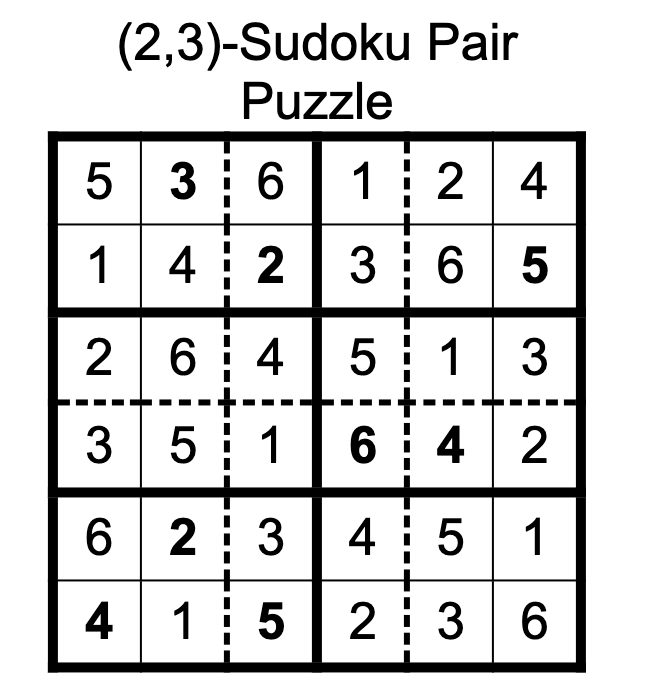
\includegraphics[width=4in]{images/23SPPExample.png}
	\end{center}
	We've been describing $(2,3)$ Sudoku pair puzzles.  A slightly harder example would be $(2,5)$ Sudoku pair puzzles. There are many variations of these puzzles that were originally designed by Dr. James Hammer in 2012. We have these puzzles on our webpage (\href{https://open-math-book.github.io/MWAU/23spp/index.html}{https://open-math-book.github.io/MWAU/23spp/index.html} for the $(2,3)$ Sudoku pair puzzles) that will allow you to generate and practice on multiple games. 
	

	
	\Instr{The $(2,5)$ Sudoku pair puzzles are often too hard for these students, so you may ask them to complete a $(2,3)$ version only.}
\end{enumerate}

\Instr{ The following pages have Minesweeper games in progress, Nonogram boards, KenKen puzzles, and Sudoku Pair puzzles, some with answers.\newpage

    \begin{center}
        Minesweeper Project Game 1\par\bigskip
        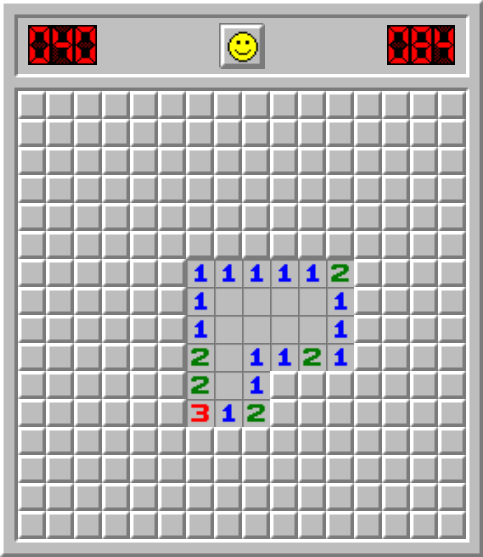
\includegraphics[width=5in]{images/MSProject1.png}
    \end{center}
    \newpage
    \begin{center}
        Minesweeper Project Game 2\par\bigskip
		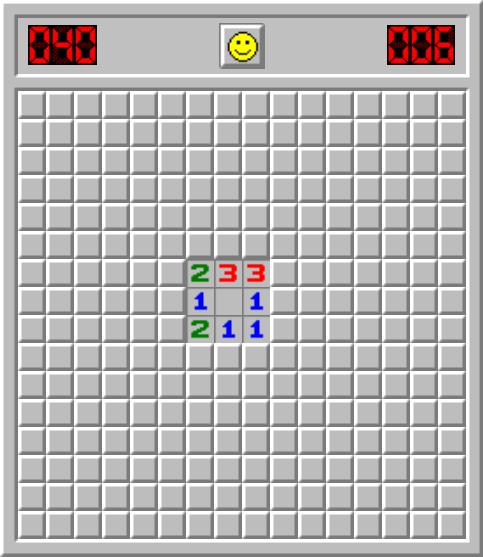
\includegraphics[width=5in]{images/MSProject2.png}
    \end{center}
    \newpage
    \begin{center}
        Minesweeper Project Game 3\par\bigskip
		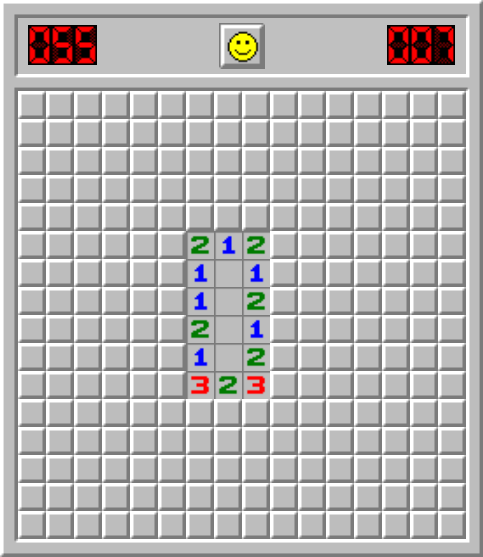
\includegraphics[width=5in]{images/MSProject3.png}
    \end{center}
    \newpage
    \begin{center}
        Minesweeper Project Game 4\par\bigskip
		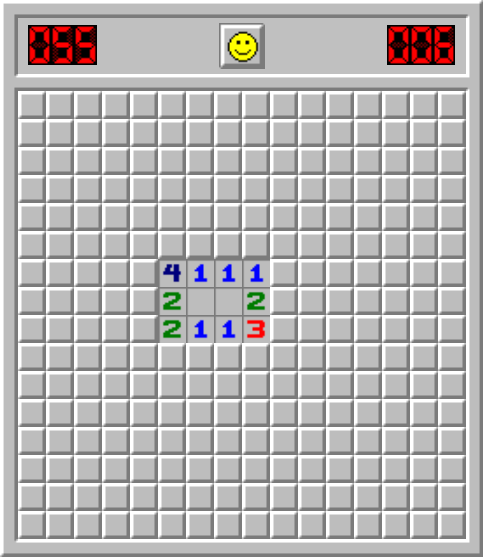
\includegraphics[width=5in]{images/MSProject4.png}
    \end{center}  
    \newpage
    \begin{center}
        Minesweeper Project Game 5\par\bigskip
		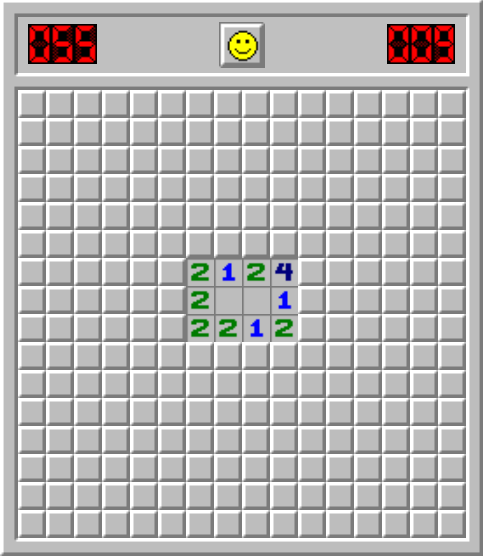
\includegraphics[width=5in]{images/MSProject5.png}
    \end{center}
    \newpage
    \begin{center}
        Minesweeper Project Game 6\par\bigskip
		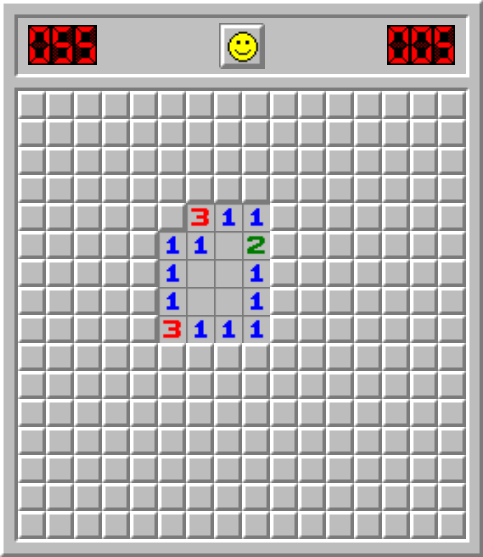
\includegraphics[width=5in]{images/MSProject6.png}
    \end{center}
    \newpage
    \begin{center}
        Minesweeper Project Game 7\par\bigskip
		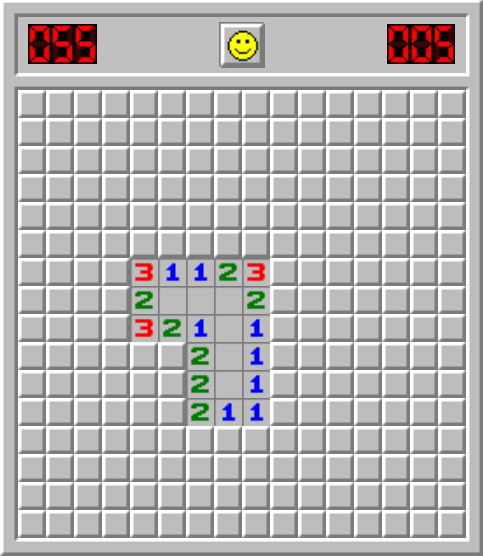
\includegraphics[width=5in]{images/MSProject7.png}
    \end{center}
    \newpage
    \begin{center}
        Minesweeper Project Game 8\par\bigskip
		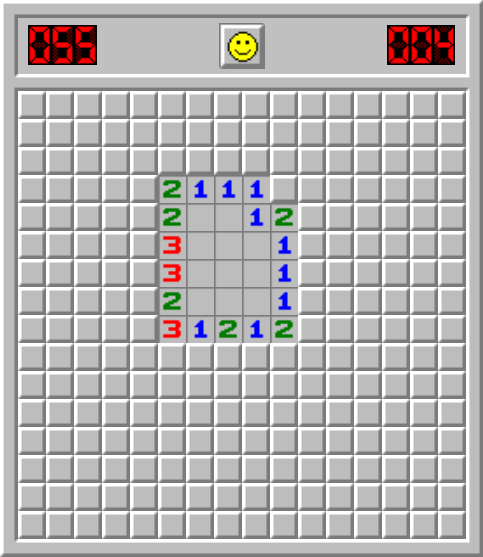
\includegraphics[width=5in]{images/MSProject8.png}
    \end{center}
    \newpage
    \begin{center}
        Minesweeper Project Game 9\par\bigskip
		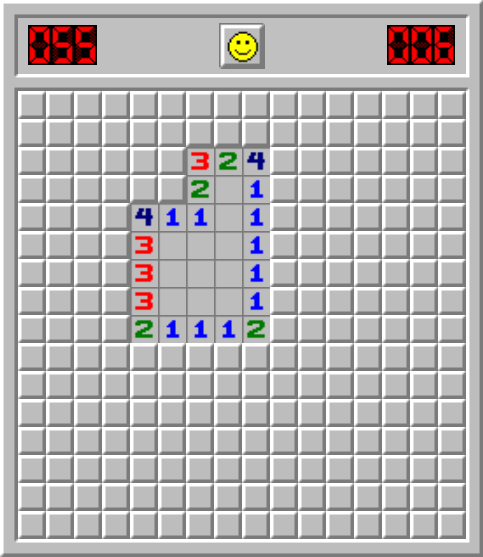
\includegraphics[width=5in]{images/MSProject9.png}
    \end{center}
    \newpage
    \begin{center}
        Minesweeper Project Game 10\par\bigskip
		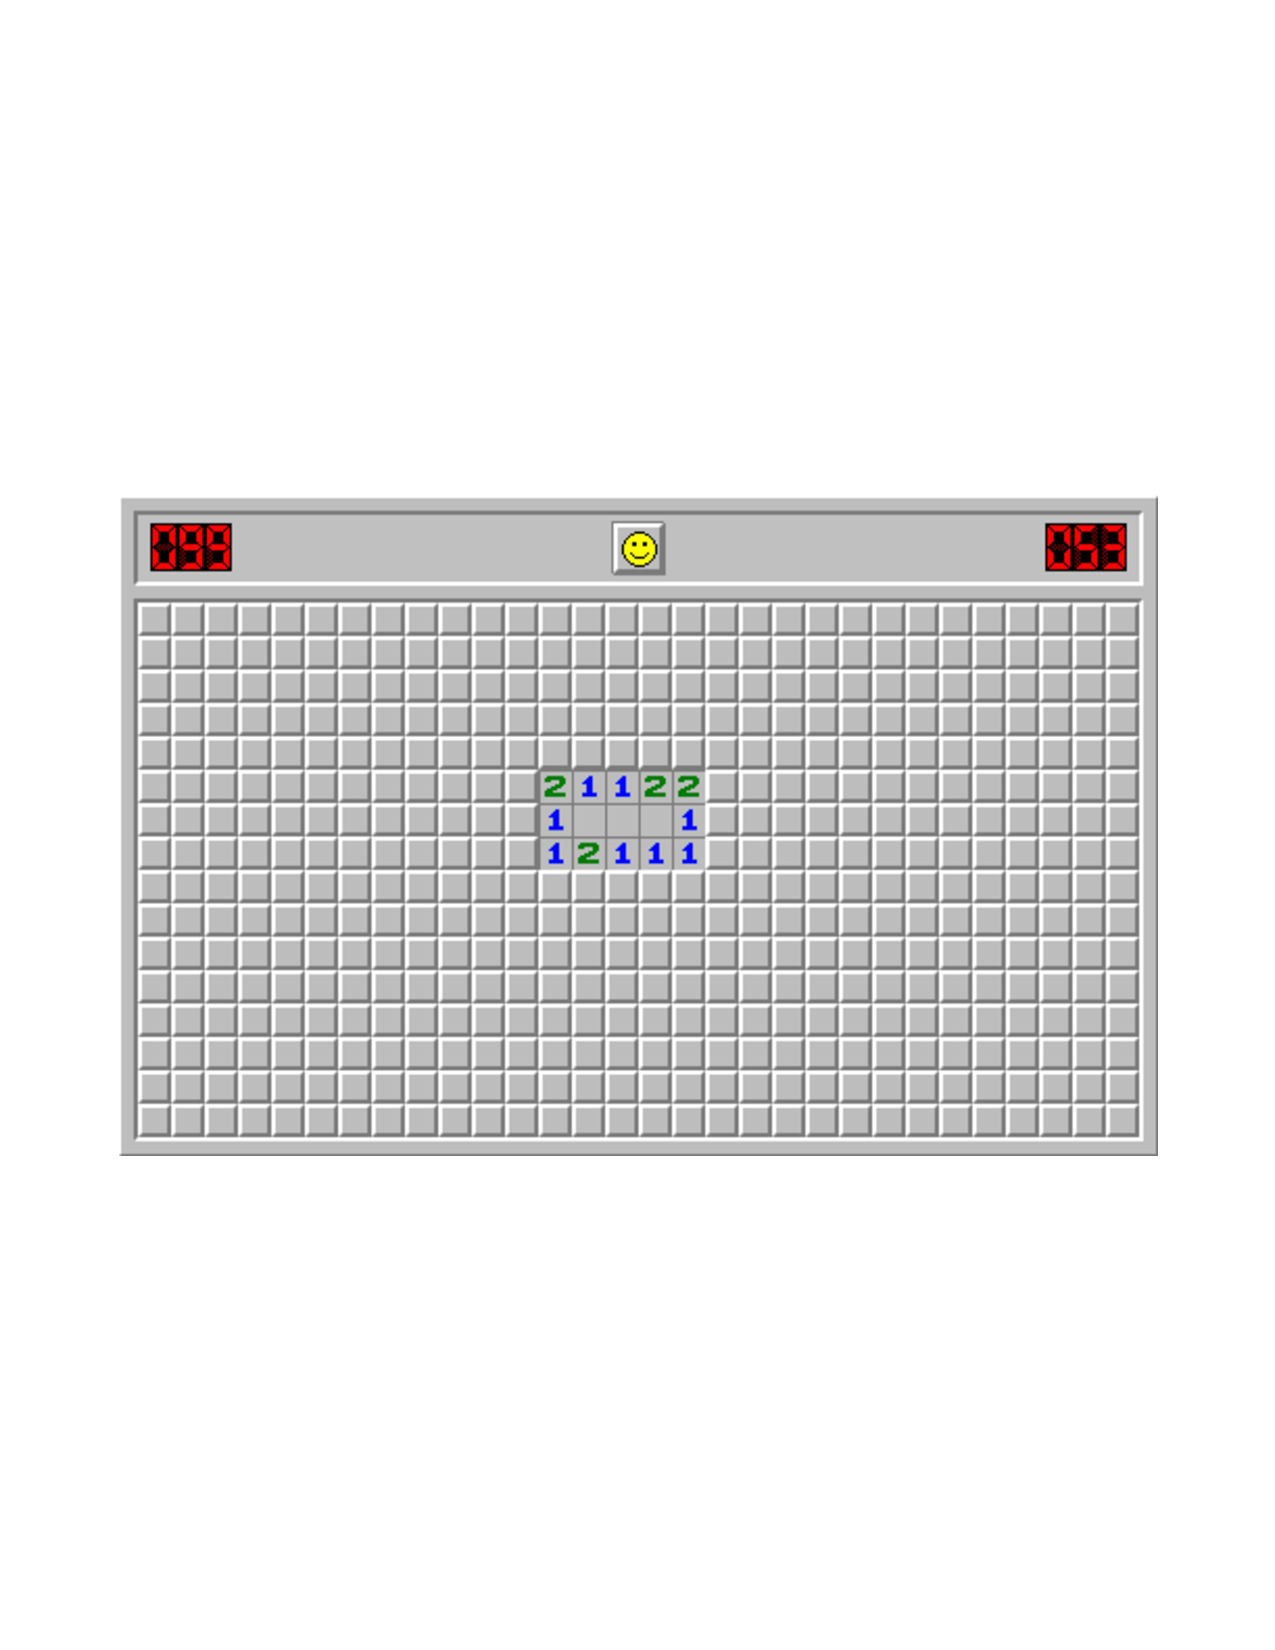
\includegraphics[width=6in]{images/MinesweeperSurrounded.pdf}
    \end{center}

    \newpage
    \begin{center}
        Nonogram Project Board 1\par\bigskip
        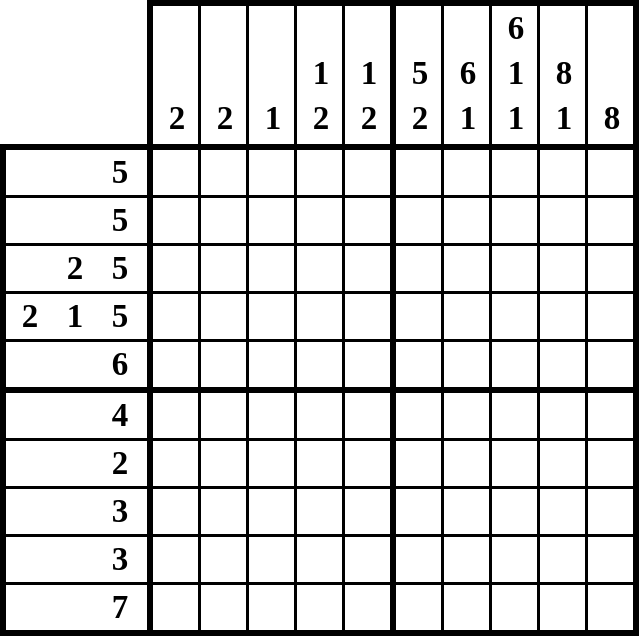
\includegraphics[width=5in]{images/nonogram01.png}
    \end{center}
    \newpage
    \begin{center}
        Nonogram Project Board 2\par\bigskip
        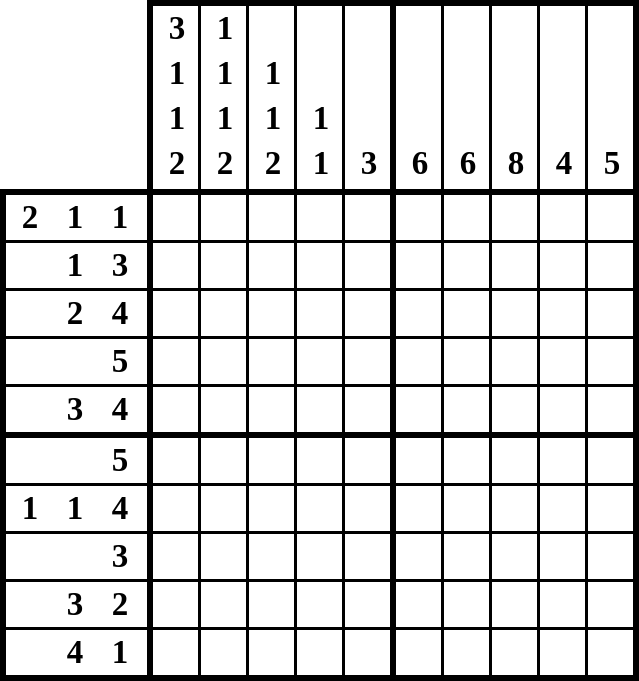
\includegraphics[width=5in]{images/nonogram02.png}
    \end{center}
    \newpage
    \begin{center}
        Nonogram Project Board 3\par\bigskip
        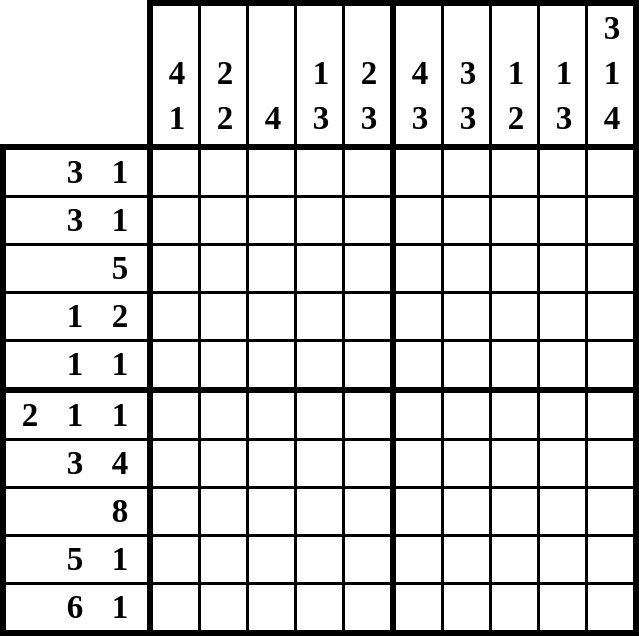
\includegraphics[width=5in]{images/nonogram03.png}
    \end{center}
    \newpage
    \begin{center}
        Nonogram Project Board 4\par\bigskip
        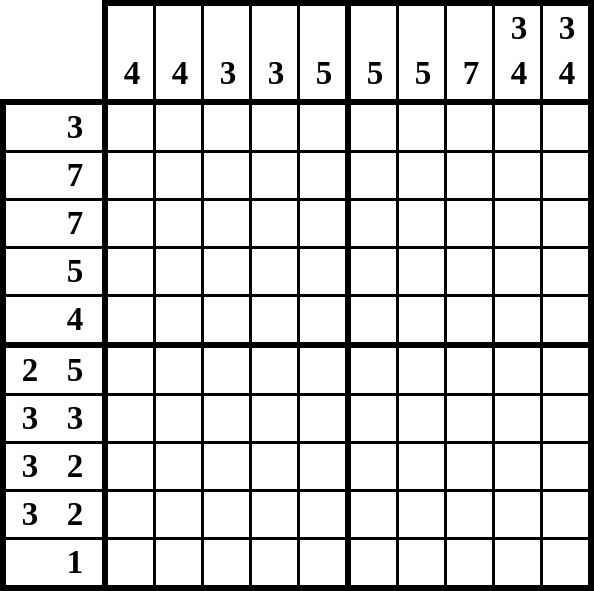
\includegraphics[width=5in]{images/nonogram04.png}
    \end{center}
    \newpage
    \begin{center}
        Nonogram Project Board 5\par\bigskip
        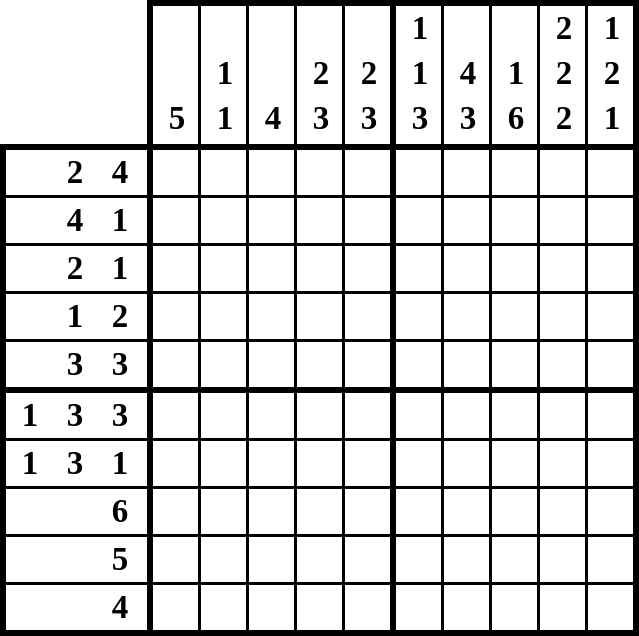
\includegraphics[width=5in]{images/nonogram05.png}
    \end{center}
    \newpage
    \begin{center}
        Nonogram Project Board 6\par\bigskip
        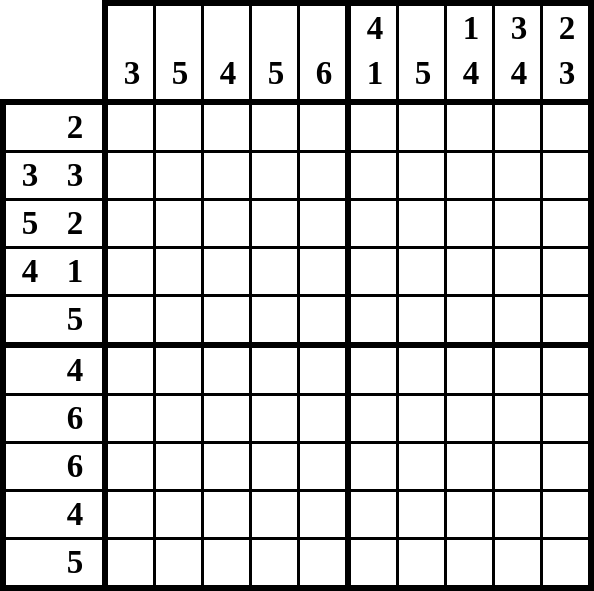
\includegraphics[width=5in]{images/nonogram06.png}
    \end{center}
    \newpage
    \begin{center}
        Nonogram Project Board 7\par\bigskip
        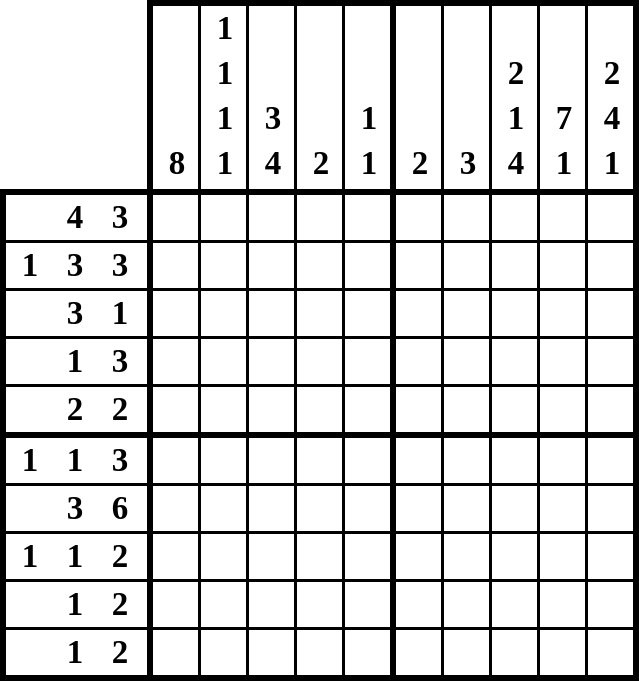
\includegraphics[width=5in]{images/nonogram07.png}
    \end{center}
    \newpage
    \begin{center}
        Nonogram Project Board 8\par\bigskip
        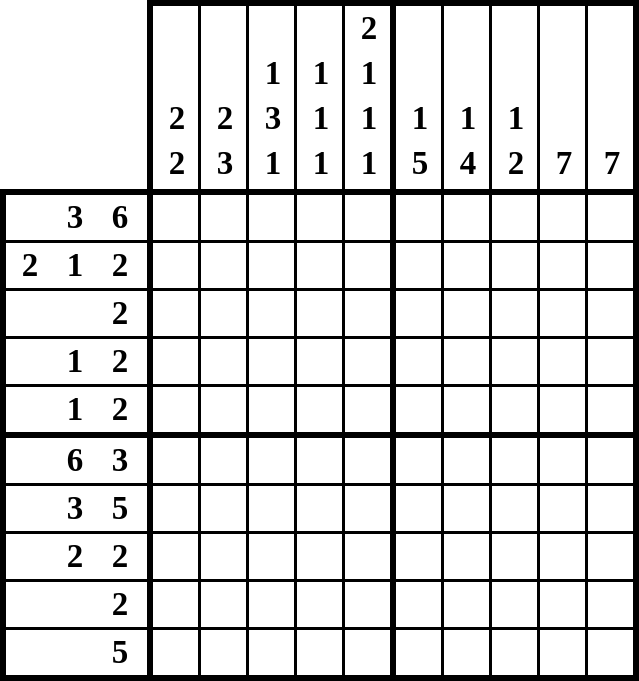
\includegraphics[width=5in]{images/nonogram08.png}
    \end{center}
    \newpage
    \begin{center}
        Nonogram Project Board 9\par\bigskip
        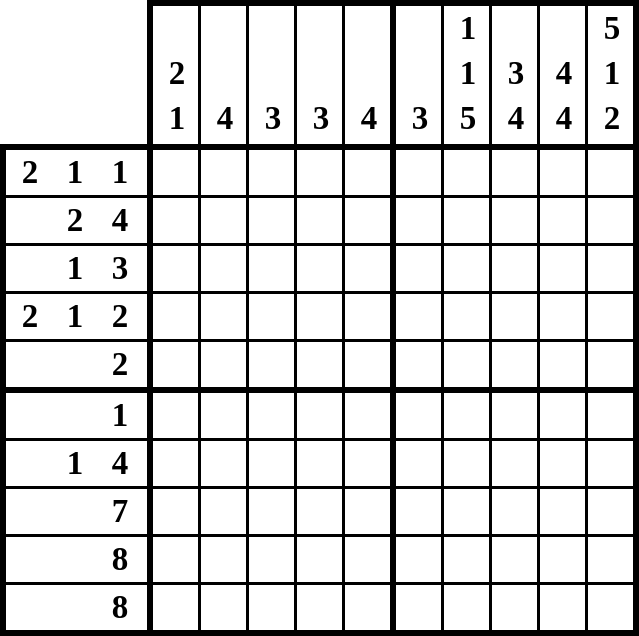
\includegraphics[width=5in]{images/nonogram09.png}
    \end{center}
    \newpage
    \begin{center}
        Nonogram Project Board 10\par\bigskip
        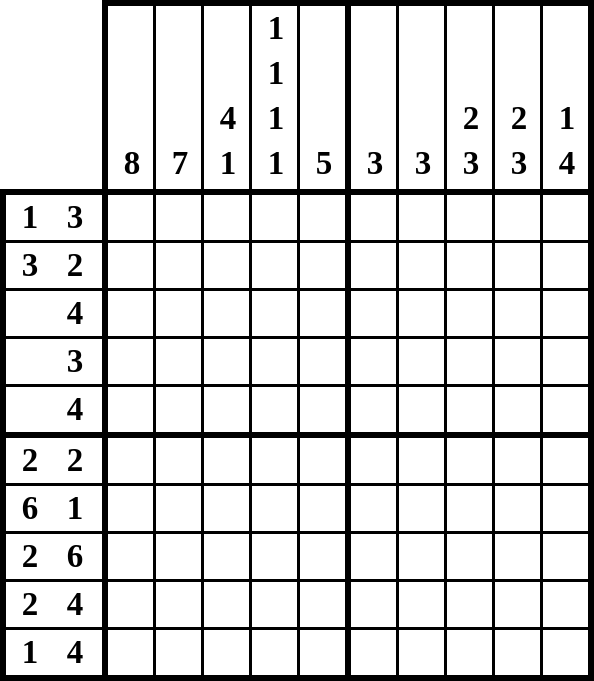
\includegraphics[width=5in]{images/nonogram10.png}
    \end{center}

    \newpage
    \begin{center}
        KenKen Project Puzzles 1\par\bigskip
        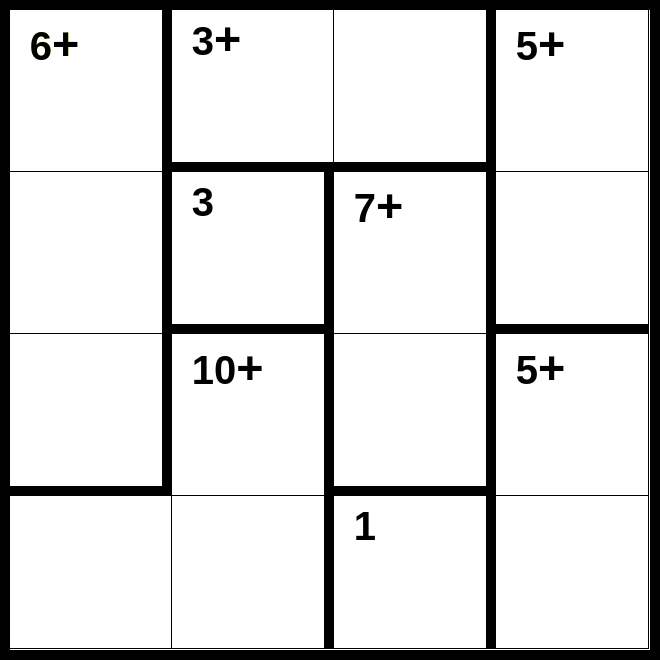
\includegraphics[width=2.8in]{images/kenken01a.png}\vfill
        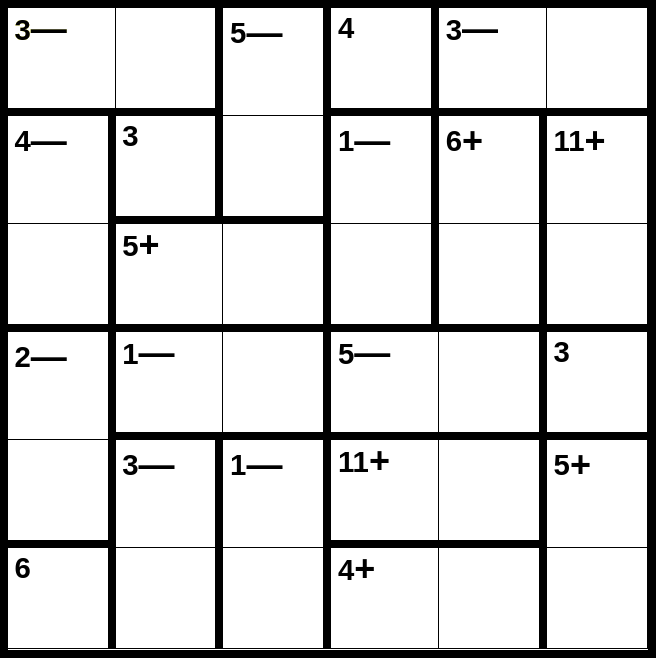
\includegraphics[width=4.2in]{images/kenken01b.png}\vfill
    \end{center}
    \newpage
    \begin{center}
        KenKen Project Puzzles 2\par\bigskip
        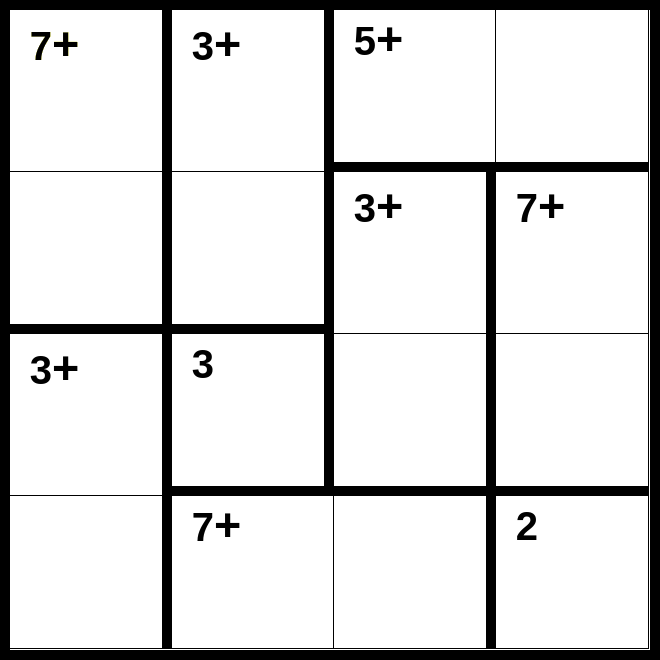
\includegraphics[width=2.8in]{images/kenken02a.png}\vfill
        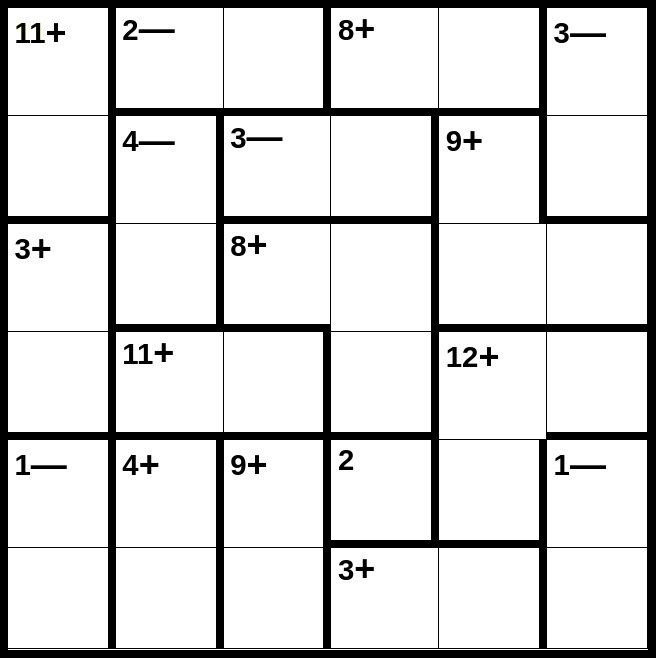
\includegraphics[width=4.2in]{images/kenken02b.png}\vfill
    \end{center}
    \newpage
    \begin{center}
        KenKen Project Puzzles 3\par\bigskip
        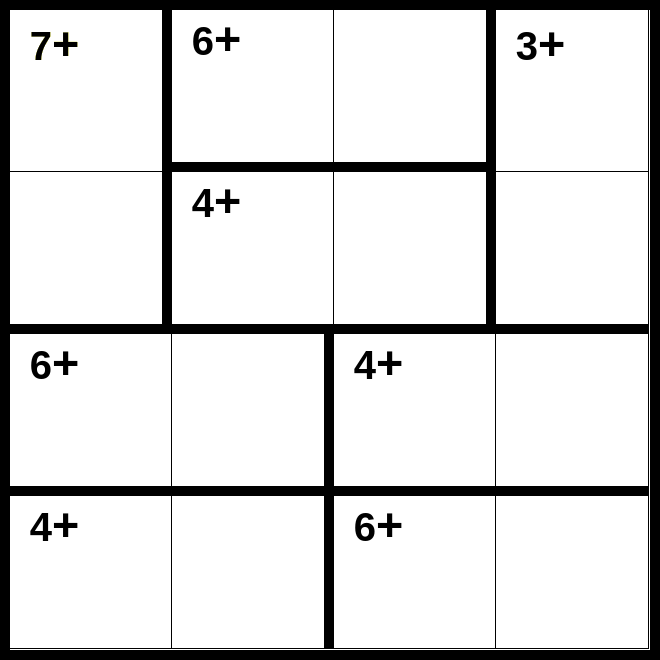
\includegraphics[width=2.8in]{images/kenken03a.png}\vfill
        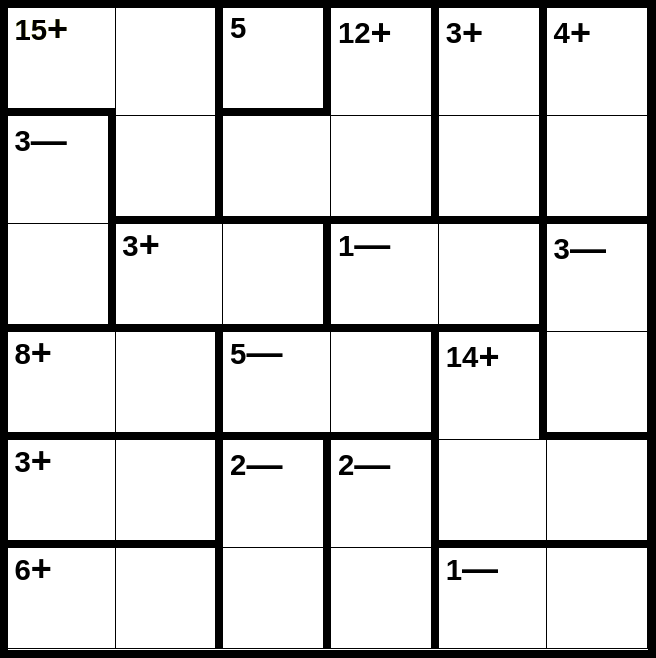
\includegraphics[width=4.2in]{images/kenken03b.png}\vfill
    \end{center}
    \newpage
    \begin{center}
        KenKen Project Puzzles 4\par\bigskip
        \includegraphics[width=2.8in]{images/kenken04a.png}\vfill
        \includegraphics[width=4.2in]{images/kenken04b.png}\vfill
    \end{center}
    \newpage
    \begin{center}
        KenKen Project Puzzles 5\par\bigskip
        \includegraphics[width=2.8in]{images/kenken05a.png}\vfill
        \includegraphics[width=4.2in]{images/kenken05b.png}\vfill
    \end{center}
    \newpage
    \begin{center}
        KenKen Project Puzzles 6\par\bigskip
        \includegraphics[width=2.8in]{images/kenken06a.png}\vfill
        \includegraphics[width=4.2in]{images/kenken06b.png}\vfill
    \end{center}
    \newpage
    \begin{center}
        KenKen Project Puzzles 7\par\bigskip
        \includegraphics[width=2.8in]{images/kenken07a.png}\vfill
        \includegraphics[width=4.2in]{images/kenken07b.png}\vfill
    \end{center}
    \newpage
    \begin{center}
        KenKen Project Puzzles 8\par\bigskip
        \includegraphics[width=2.8in]{images/kenken08a.png}\vfill
        \includegraphics[width=4.2in]{images/kenken08b.png}\vfill
    \end{center}
    \newpage
    \begin{center}
        KenKen Project Puzzles 9\par\bigskip
        \includegraphics[width=2.8in]{images/kenken09a.png}\vfill
        \includegraphics[width=4.2in]{images/kenken09b.png}\vfill
    \end{center}
    \newpage
    \begin{center}
        KenKen Project Puzzles 10\par\bigskip
        \includegraphics[width=2.8in]{images/kenken10a.png}\vfill
        \includegraphics[width=4.2in]{images/kenken10b.png}\vfill
    \end{center}

\newpage
\begin{center}
        (2,3) - Sudoku Pair Puzzle 1
        
    \includegraphics[width=5in]{images/SPP23-01.png}
      \end{center}

\newpage
\begin{center}
        (2,3) - Sudoku Pair Puzzle 2
        
    \includegraphics[width=5in]{images/SPP23-02.png}
      \end{center}


\newpage
\begin{center}
        (2,3) - Sudoku Pair Puzzle 3
        
    \includegraphics[width=5in]{images/SPP23-03.png}
      \end{center}


\newpage
\begin{center}
        (2,3) - Sudoku Pair Puzzle 4
        
    \includegraphics[width=5in]{images/SPP23-04.png}
      \end{center}



\newpage
\begin{center}
        (2,3) - Sudoku Pair Puzzle 5
        
    \includegraphics[width=5in]{images/SPP23-05.png}
      \end{center}


\newpage
\begin{center}
        (2,3) - Sudoku Pair Puzzle 6
        
    \includegraphics[width=5in]{images/SPP23-06.png}
      \end{center}


\newpage
\begin{center}
        (2,3) - Sudoku Pair Puzzle 7
        
    \includegraphics[width=5in]{images/SPP23-07.png}
      \end{center}


\newpage
\begin{center}
        (2,3) - Sudoku Pair Puzzle 8
        
    \includegraphics[width=5in]{images/SPP23-08.png}
      \end{center}


\newpage
\begin{center}
        (2,3) - Sudoku Pair Puzzle 9
        
    \includegraphics[width=5in]{images/SPP23-09.png}
      \end{center}


\newpage
\begin{center}
        (2,3) - Sudoku Pair Puzzle 10
        
    \includegraphics[width=5in]{images/SPP23-10.png}
      \end{center}





\newpage
\begin{center}
        (2,5) - Sudoku Pair Puzzle 1
        
    \includegraphics[width=5in]{images/SPP1.png}
      \end{center}

\newpage
\begin{center}
        (2,5) - Sudoku Pair Puzzle 2
        
    \includegraphics[width=5in]{images/SPP2.png}
      \end{center}


\newpage
\begin{center}
        (2,5) - Sudoku Pair Puzzle 3
        
    \includegraphics[width=5in]{images/SPP3.png}
      \end{center}



\newpage
\begin{center}
        (2,5) - Sudoku Pair Puzzle 4
        
    \includegraphics[width=5in]{images/SPP4.png}
      \end{center}



\newpage
\begin{center}
        (2,5) - Sudoku Pair Puzzle 5
        
    \includegraphics[width=5in]{images/SPP5.png}
      \end{center}


\newpage
\begin{center}
        (2,5) - Sudoku Pair Puzzle 6
        
    \includegraphics[width=5in]{images/SPP6.png}
      \end{center}


\newpage
\begin{center}
        (2,5) - Sudoku Pair Puzzle 7
        
    \includegraphics[width=5in]{images/SPP7.png}
      \end{center}


\newpage
\begin{center}
        (2,5) - Sudoku Pair Puzzle 8
        
    \includegraphics[width=5in]{images/SPP8.png}
      \end{center}


\newpage
\begin{center}
        (2,5) - Sudoku Pair Puzzle 9
        
    \includegraphics[width=5in]{images/SPP9.png}
      \end{center}


\newpage
\begin{center}
        (2,5) - Sudoku Pair Puzzle 10
        
    \includegraphics[width=5in]{images/SPP10.png}
      \end{center}



\newpage
\begin{center}
        (2,5) - Sudoku Pair Puzzle Solution 1
        
    \includegraphics[width=5in]{images/SPP1Solved.png}
      \end{center}

\newpage
\begin{center}
        (2,5) - Sudoku Pair Puzzle Solution 1
        
    \includegraphics[width=5in]{images/SPP1Solved.png}
      \end{center}

\newpage
\begin{center}
        (2,5) - Sudoku Pair Puzzle Solution 2
        
    \includegraphics[width=5in]{images/SPP2Solved.png}
      \end{center}
    
\newpage
\begin{center}
        (2,5) - Sudoku Pair Puzzle Solution 3
        
    \includegraphics[width=5in]{images/SPP3Solved.png}
      \end{center}

\newpage
\begin{center}
        (2,5) - Sudoku Pair Puzzle Solution 4
        
    \includegraphics[width=5in]{images/SPP4Solved.png}
      \end{center}
\newpage

\newpage
\begin{center}
        (2,5) - Sudoku Pair Puzzle Solution 5
        
    \includegraphics[width=5in]{images/SPP5Solved.png}
      \end{center}

\newpage
\begin{center}
        (2,5) - Sudoku Pair Puzzle Solution 6
        
    \includegraphics[width=5in]{images/SPP6Solved.png}
      \end{center}
      
\newpage
\begin{center}
        (2,5) - Sudoku Pair Puzzle Solution 7
        
    \includegraphics[width=5in]{images/SPP7Solved.png}
      \end{center}

\newpage
\begin{center}
        (2,5) - Sudoku Pair Puzzle Solution 8
        
    \includegraphics[width=5in]{images/SPP8Solved.png}
      \end{center}


\newpage
\begin{center}
        (2,5) - Sudoku Pair Puzzle Solution 9
        
    \includegraphics[width=5in]{images/SPP9Solved.png}
      \end{center}

\newpage
\begin{center}
        (2,5) - Sudoku Pair Puzzle Solution 10
        
    \includegraphics[width=5in]{images/SPP10Solved.png}
      \end{center}
}

\newpage
%<*truthTables:exercises:title>
\section{Additional Exercises}
%</truthTables:exercises:title>

%<*truthTables:exercises:conTTableA>
\begin{enumerate}
\item Construct a truth table\index{truth table} for the following statements\index{statement}. \index{$\vee$}\index{$\wedge$}\index{$\neg$}\index{$\Rightarrow$}
\begin{enumerate}
\item $\neg(\neg P \wedge \neg Q)$
%</truthTables:exercises:conTTableA>

\Instr{ 
\begin{center}
\begin{tabular}{|c|c||c|}
\hline
$P$ & $Q$ & $\neg(\neg P\wedge \neg Q)$ \\
\hline
\hline
True & True & True \\
\hline
True & False & True \\
\hline
False & True & True \\
\hline
False & False & False \\
\hline
\end{tabular}
\end{center}
}

%<*truthTables:exercises:conTTableB>
\item $\neg(\neg P \vee \neg Q)$
%</truthTables:exercises:conTTableB>

\Instr{ 
\begin{center}
\begin{tabular}{|c|c||c|}
\hline
$P$ & $Q$ & $\neg(\neg P \vee \neg Q)$ \\
\hline
\hline
True & True & True \\
\hline
True & False & False \\
\hline
False & True & False \\
\hline
False & False & False \\
\hline
\end{tabular}
\end{center}
}

%<*truthTables:exercises:conTTableC>
\item $\neg(P\Rightarrow \neg Q)$
%</truthTables:exercises:conTTableC>

\Instr{ 

\begin{center}
\begin{tabular}{|c|c||c|}
\hline
$P$ & $Q$ & $\neg(P\Rightarrow \neg Q)$ \\
\hline
\hline
True & True & True \\
\hline
True & False & False \\
\hline
False & True & False \\
\hline
False & False & False \\
\hline
\end{tabular}
\end{center}
}

%<*truthTables:exercises:conTTableD>
\item $(P\vee Q)\Rightarrow P$
%</truthTables:exercises:conTTableD>

\Instr{ 
\begin{center}
\begin{tabular}{|c|c||c|}
\hline
$P$ & $Q$ & $(P\vee Q)\Rightarrow P$ \\
\hline
\hline
True & True & True \\
\hline
True & False & True \\
\hline
False & True & False \\
\hline
False & False & True \\
\hline
\end{tabular}
\end{center}
}

%<*truthTables:exercises:endifAndOnlyIf>
\end{enumerate}

\item\label{ifAndOnlyIf} The $\Leftrightarrow$ operator is known as the ``if and only if'' operator and is defined to be the statement $(P\Rightarrow Q)\wedge (Q\Rightarrow P)$. Its truth table is given in Table~{\normalfont\ref{iffTable}}. Find a way to write the statement $P\Leftrightarrow Q$\index{$\Leftrightarrow$} using the statements $P$ and $Q$, and the operators $\neg$, $\vee$, or $\wedge$. ({\em Hint}: Construct a truth table first.)

\begin{table}[H]
\begin{center}
\begin{tabular}{|c|c||c|}
\hline
$P$ & $Q$ & $P\Leftrightarrow Q$ \\
\hline
\hline
True & True & True \\
\hline
True & False & False \\
\hline
False & True & False \\
\hline
False & False & True \\
\hline
\end{tabular}
\end{center}
\caption{Truth table for $\Leftrightarrow$ operator}\label{iffTable}
\end{table}
%</truthTables:exercises:endifAndOnlyIf>

\Instr{  By constructing a truth table, it is easy to see $(P\wedge Q)\vee(\neg P\wedge \neg Q)$ is equivalent to $P\Leftrightarrow Q$.
}

%<*truthTables:exercises:conMoreTTableA>
\item Construct a truth table for the following statements\index{statement}\index{$\neg$}\index{$\wedge$}\index{$\vee$}\index{$\Rightarrow$}\index{$\Leftrightarrow$}.
\begin{enumerate}
\item $\neg P\Leftrightarrow P$
%</truthTables:exercises:conMoreTTableA>

\Instr{ 
\begin{center}
\begin{tabular}{|c|c||c|}
\hline
$P$ & $Q$ & $\neg P \Leftrightarrow P$ \\
\hline
\hline
True & True & False \\
\hline
True & False & False \\
\hline
False & True & False \\
\hline
False & False & False \\
\hline
\end{tabular}
\end{center}
}

%<*truthTables:exercises:conMoreTTableB>
\item $\neg (P\vee Q) \Leftrightarrow (\neg P\wedge \neg Q)$ 
%</truthTables:exercises:conMoreTTableB>

\Instr{ 
\begin{center}
\begin{tabular}{|c|c||c|}
\hline
$P$ & $Q$ & $\neg (P\vee Q) \Leftrightarrow (\neg P\wedge \neg Q)$ \\
\hline
\hline
True & True & True \\
\hline
True & False & True \\
\hline
False & True & True \\
\hline
False & False & True \\
\hline
\end{tabular}
\end{center}
}

%<*truthTables:exercises:conMoreTTableC>
\item $\neg(P\Rightarrow Q)\Rightarrow (\neg Q\Rightarrow P)$
%</truthTables:exercises:conMoreTTableC>

\Instr{ 
\begin{center}
\begin{tabular}{|c|c||c|}
\hline
$P$ & $Q$ & $\neg(P\Rightarrow Q)\Rightarrow (\neg Q\Rightarrow P)$ \\
\hline
\hline
True & True & True \\
\hline
True & False & True \\
\hline
False & True & True \\
\hline
False & False & True \\
\hline
\end{tabular}
\end{center}
}

%<*truthTables:exercises:conMoreTTableD>
\item $((P\Leftrightarrow Q)\wedge (P\Rightarrow R))\vee (\neg P\Rightarrow (Q\wedge R))$
%</truthTables:exercises:conMoreTTableD>

\Instr{ 
\begin{center}
\begin{tabular}{|c|c|c||c|}
\hline
$P$ & $Q$ & $R$ & $((P\Leftrightarrow Q)\wedge (P\Rightarrow R))\vee (\neg P\Rightarrow (Q\wedge R))$ \\
\hline
\hline
True & True & True & True \\
\hline
True & True & False & True \\
\hline
True & False & True & True \\
\hline
True & False & False & True \\
\hline
False & True & True & True \\
\hline
False & True & False & False \\
\hline
False & False & True & True \\
\hline
False & False & False & True \\
\hline
\end{tabular}
\end{center}
}

%<*truthTables:exercises:conMoreTTableE>
\item $\neg (\neg P\Rightarrow (Q\vee R))\Rightarrow (\neg P \wedge Q)$
%</truthTables:exercises:conMoreTTableE>

\Instr{ 
\begin{center}
\begin{tabular}{|c|c|c||c|}
\hline
$P$ & $Q$ & $R$ & $\neg (\neg P\Rightarrow (Q\vee R))\Rightarrow (\neg P \wedge Q)$ \\
\hline
\hline
True & True & True & True \\
\hline
True & True & False & True \\
\hline
True & False & True & True \\
\hline
True & False & False & True \\
\hline
False & True & True & True \\
\hline
False & True & False & True \\
\hline
False & False & True & False \\
\hline
False & False & False & False \\
\hline
\end{tabular}
\end{center}
}
%<*truthTables:exercises:endTautology>
\end{enumerate}

\item Write a single statement using $P$, $Q$, and $R$ along with the symbols $\neg$, $\vee$, $\wedge$, or $\Rightarrow$ that is always true.
%</truthTables:exercises:endTautology>

\Instr{  
There are many solutions to this question. One such statement is $((P\vee Q)\vee R)\vee \neg P$. Any statement that is always true is called a \textbf{tautology}\index{tautology}.
}

%<*truthTables:exercises:stateJake>
\item Consider the following statements about Jake. 

\begin{minipage}[H]{5.75in}
\tt
\begin{center}
{ ``If today is Wednesday, then Jake's class has library day. If Jake's class has library day, then Jake will bring home a new book. Jake did not bring any new books home today.''}
\end{center}
\end{minipage}

What can you conclude based on the given information? Explain your answer.
%</truthTables:exercises:stateJake>

\Instr{  Since Jake did not bring a book home we can assume that Jake's class did not have library day. Also, since Jake's class did not have library day, you may conclude that today must not be Wednesday. 

This can be explained in a different way using statements as well. Let the statement ``today is Wednesday'' be $P$, the statement ``Jake's class has library day'' be $Q$, and the statement ``Jake will bring home a new book'' be $R$. Then the first sentence says $P\Rightarrow Q$, the second sentence says $Q\Rightarrow R$ and the last sentence says $R$ is false. For the statement $Q\Rightarrow R$ to hold true, $Q$ must be false and so Jake's class did not have library day. Similarly, For the statement $P\Rightarrow Q$ to hold true, $P$ must be false, so today is not Wednesday.
}

%<*truthTables:exercises:equalState>
\item Show that the two statements\index{statement} $((P\wedge Q)\Rightarrow R)$\index{$\wedge$}\index{$\Rightarrow$}\index{$\neg$}\index{$\vee$} and $(\neg P)\vee (\neg Q) \vee R$ are equivalent. Give an example in which $P$, $Q$, and $R$ each stand for some statement (like in Activity~{\normalfont\ref{conditional}}, then explain what the statements $((P\wedge Q)\Rightarrow R)$ and $(\neg P)\vee (\neg Q) \vee R$ mean in your given context.
%</truthTables:exercises:equalState>

\Instr{  The following truth table shows that the statements $((P\wedge Q)\Rightarrow R)$ and $(\neg P)\vee(\neg Q)\vee R$ are equivalent.
\begin{center}
\begin{tabular}{|c|c|c||c|c|}
\hline
$P$ & $Q$ & $R$ & $((P\wedge Q)\Rightarrow R)$ & $(\neg P)\vee (\neg Q)\vee R$ \\
\hline
\hline
True & True & True & True & True \\
\hline
True & True & False & False & False \\
\hline
True & False & True & True & True \\
\hline
True & False & False & True & True \\
\hline
False & True & True & True & True \\
\hline
False & True & False & True & True \\
\hline
False & False & True & True & True \\
\hline
False & False & False & True & True \\
\hline
\end{tabular}
\end{center}

Let statement $P$ be ``I drive to work'', statement $Q$ be ``I wear brown pants'', and statement $R$ be ``I wear brown shoes.'' Then $((P\wedge Q)\Rightarrow R)$ says if I drive to work and wear brown pants, then I will wear brown shoes. The statement $(\neg P)\vee (\neg Q)\vee R$ says I will not drive to work or I will not wear brown pants or I will wear brown shoes.
}

%<*truthTables:exercises:matchTTablePreA>
\item Write out a statement\index{statement} using $P$ and $Q$ with the operators $\neg$, $\wedge$, or $\vee$ that has the indicated truth table\index{truth table}.
%</truthTables:exercises:matchTTablePreA>

\Instr{  Each question has multiple solutions. We give one possible answer.
}

%<*truthTables:exercises:matchTTableA>
\begin{enumerate}
\item \mbox{}
\begin{center}
\begin{tabular}{|c|c||c|}
\hline
$P$ & $Q$ & \hspace{1.75in} \\
\hline
\hline
True & True & True \\
\hline
True & False & True \\
\hline
False & True & False \\
\hline
False & False & True \\
\hline
\end{tabular}
\end{center}
%</truthTables:exercises:matchTTableA>

\Instr{  
\begin{center}
\begin{tabular}{|c|c||c|}
\hline
$P$ & $Q$ & $\neg Q\vee P$ \\
\hline
\hline
True & True & True \\
\hline
True & False & True \\
\hline
False & True & False \\
\hline
False & False & True \\
\hline
\end{tabular}
\end{center}
}

%<*truthTables:exercises:matchTTableB>
\item \mbox{}
\begin{center}
\begin{tabular}{|c|c||c|}
\hline
$P$ & $Q$ & \hspace{1.75in} \\
\hline
\hline
True & True & False \\
\hline
True & False & False \\
\hline
False & True & True \\
\hline
False & False & False \\
\hline
\end{tabular}
\end{center}
%</truthTables:exercises:matchTTableB>

\Instr{ 
\begin{center}
\begin{tabular}{|c|c||c|}
\hline
$P$ & $Q$ & $\neg(\neg Q\vee P)=Q\wedge \neg P$ \\
\hline
\hline
True & True & False \\
\hline
True & False & False \\
\hline
False & True & True \\
\hline
False & False & False \\
\hline
\end{tabular}
\end{center}
}

%<*truthTables:exercises:matchTTableC>
\item \mbox{}
\begin{center}
\begin{tabular}{|c|c||c|}
\hline
$P$ & $Q$ & \hspace{1.75in} \\
\hline
\hline
True & True & True \\
\hline
True & False & True \\
\hline
False & True & True \\
\hline
False & False & True \\
\hline
\end{tabular}
\end{center}
%</truthTables:exercises:matchTTableC>

\Instr{  
\begin{center}
\begin{tabular}{|c|c||c|}
\hline
$P$ & $Q$ & $(P\vee Q)\vee \neg P$ \\
\hline
\hline
True & True & True \\
\hline
True & False & True \\
\hline
False & True & True \\
\hline
False & False & True \\
\hline
\end{tabular}
\end{center}
}

%<*truthTables:exercises:matchTTableD>
\item \mbox{}
\begin{center}
\begin{tabular}{|c|c||c|}
\hline
$P$ & $Q$ & \hspace{1.75in} \\
\hline
\hline
True & True & True \\
\hline
True & False & True \\
\hline
False & True & True \\
\hline
False & False & False \\
\hline
\end{tabular}
\end{center}
%</truthTables:exercises:matchTTableD>

\Instr{  
\begin{center}
\begin{tabular}{|c|c||c|}
\hline
$P$ & $Q$ & $P\vee Q$ \\
\hline
\hline
True & True & True \\
\hline
True & False & True \\
\hline
False & True & True \\
\hline
False & False & False \\
\hline
\end{tabular}
\end{center}
}

%<*truthTables:exercises:matchTTableE>
\item \mbox{}
\begin{center}
\begin{tabular}{|c|c||c|}
\hline
$P$ & $Q$ & \hspace{1.75in} \\
\hline
\hline
True & True & False \\
\hline
True & False & False \\
\hline
False & True & True \\
\hline
False & False & True \\
\hline
\end{tabular}
\end{center}
%</truthTables:exercises:matchTTableE>

\Instr{ 
\begin{center}
\begin{tabular}{|c|c||c|}
\hline
$P$ & $Q$ & $\neg P$ or $\neg P \wedge (\neg P\vee \neg Q)$ \\
\hline
\hline
True & True & False \\
\hline
True & False & False \\
\hline
False & True & True \\
\hline
False & False & True \\
\hline
\end{tabular}
\end{center}
}
%<*truthTables:exercises:endOplus>
\end{enumerate}

\item The $\oplus$ symbol is known as XOR and is the statement that is true if exactly one of $P$ and $Q$ is true. Its truth table is given in Table~{\normalfont\ref{xorTable}}. Write a statement that is equivalent to $P\oplus Q$\index{$\oplus$} using the symbols $\neg$, $\vee$, or $\wedge$. 

\begin{table}[H]
\begin{center}
\begin{tabular}{|c|c||c|}
\hline
$P$ & $Q$ & $P\oplus Q$ \\
\hline
\hline
True & True & False \\
\hline
True & False & True \\
\hline
False & True & True \\
\hline
False & False & False \\
\hline
\end{tabular}
\end{center}
\caption{Truth table for $\oplus$ symbol}\label{xorTable}
\end{table}
%</truthTables:exercises:endOplus>

\Instr{  By constructing a truth table, it is easy to see $(P\vee Q)\wedge \neg(P\wedge Q)$ is equivalent to $P\oplus Q$. There are other solutions as well.
}

%<*truthTables:exercises:stateMoreEqualA>
\item Show that the pair of statements\index{statement} are equivalent using truth tables\index{truth table}.
\begin{enumerate}
\item $\neg (P \wedge Q)$ and $\neg P \vee \neg Q$
%</truthTables:exercises:stateMoreEqualA>

\Instr{  
\begin{center}
\begin{tabular}{|c|c||c|c|}
\hline
$P$ & $Q$ & $\neg(P\wedge Q)$ & $\neg P \vee \neg Q$ \\
\hline
\hline
True & True & False & False \\
\hline
True & False & True & True \\
\hline
False & True & True & True \\
\hline
False & False & True & True \\
\hline
\end{tabular}
\end{center}
}

%<*truthTables:exercises:stateMoreEqualB>
\item $((P\vee Q)\wedge (\neg P)) \wedge Q$ and $\neg P\wedge Q$\index{$\wedge$}\index{$\vee$}\index{$\neg$}
%</truthTables:exercises:stateMoreEqualB>

\Instr{ 
\begin{center}
\begin{tabular}{|c|c||c|c|}
\hline
$P$ & $Q$ & $((P\vee Q)\wedge(\neg P))\wedge Q$ & $\neg P\wedge Q$ \\
\hline
\hline
True & True & False & False \\
\hline
True & False & False & False \\
\hline
False & True & True & True \\
\hline
False & False & False & False \\
\hline
\end{tabular}
\end{center}
}
%<*truthTables:exercises:endTrueLie>
\end{enumerate}

\item\label{trueLie} During your voyage across the $7$ seas you come across an island that is populated by two tribes: monks and peasants (or so they call themselves). From your interaction with them you realize that the monks always tell the truth while the peasants tell nothing but lies. Unfortunately, you cannot tell the inhabitants apart from each other. One day, two of the inhabitants, let us call them Amber and Betty, came up to you to tell you something:
\begin{itemize}
\item[] Amber says ``Exactly one of us is a monk.''
\item[] Betty says ``Only a peasant would say that Amber is a peasant.''
\end{itemize}
Can you determine to which tribe each of Amber and Betty belong?
%</truthTables:exercises:endTrueLie>

\Instr{ 
Let $A$ represent the statement made by Amber and $B$ represent the statement made by Betty. 

Suppose $A$ is true. Then either Amber or Betty is a monk but not both. Since $A$ is true, it follows that Amber is a monk, and so make Betty the peasant. Before we jump to any conclusions and declare a solution, we need to make sure Betty's statement makes sense knowing that her statement is false. Since $B$ is false, it is not true that a peasant would say that Amber is a peasant, but this is a contradiction. 

Suppose $A$ is false. Then Amber is a peasant and it is not true that either Amber or Betty is a monk but not both. So either Amber and Betty are both peasants or are both monks. Since Amber is a peasant, Betty is peasant. Finally, we must check that it makes sense that $B$ is false. Since $B$ is false, it is not true that a peasant would say that Amber is a peasant. Since Amber is a peasant it would make sense that statement $B$ is false. So both Amber and Betty are both peasants.
}

%<*truthTables:exercises:anotherTrueLie>
\item You meet another inhabitant of island described in Question~{\normalfont\ref{trueLie}}. You ask an inhabitant if there is gold on the island. He tells you ``There is gold on this island if and only if I am a monk.'' Translate this statement\index{statement} into a logical symbol. Is this person a monk or peasant? Is there gold on the island. ({\em Hint}: The ``if and only if'' operator ($\Leftrightarrow$) is discussed in Question~{\normalfont\ref{ifAndOnlyIf}}.)
%</truthTables:exercises:anotherTrueLie>

\Instr{ 
Let $P$ be the statement that there is gold on this island and let $Q$ be the statement be I am a monk. So the logical statement made in the question is $P\Leftrightarrow Q$. 

Suppose the inhabitant is a peasant. Then $Q$ and the logical statement $P\Leftrightarrow Q$ are false. By examining the table in Question~{\normalfont\ref{ifAndOnlyIf}} we see that the only way this would hold is if $P$ is true. So there would be gold on the island. No contradictions were made at this time so we must see what happens when we assume that the inhabitant is a monk. 

Suppose this inhabitant is a monk. Then $Q$ and the logical statement $P\Leftrightarrow Q$ are true. By looking back at the table in Question~{\normalfont\ref{ifAndOnlyIf}} the only way $Q$ and the statement $P\Leftrightarrow Q$ are true is if $P$ is true. So there is gold on this island. Again, no breaks in logic were made. We may never know if the inhabitant is a monk or peasant, but we know for certain that there must be gold on the island.
}

%<*truthTables:exercises:newSymbol>
\item Construct a new symbol $*$ that gives true or false responses depending on whether the statements are true or false (just like $\vee$, $\wedge$, and $\Rightarrow$). Explain how it works. Fill in the first three columns of the following table to make it clear what $P*Q$ means. Then fill in the remainder of the truth table\index{truth table}.

\begin{center}
\begin{tabular}{|c|c||c|c|c|c|c||}
\hline
$P$ & $Q$ & $P*Q$ & $((P * Q)\wedge P)\Rightarrow Q$ & $((P\Rightarrow \neg Q) *Q)\Rightarrow \neg P$ & $P*Q \Rightarrow P$  \\
\hline
\hline
\hspace{.4in} & \hspace{.4in} & \hspace{.4in} & \hspace{.4in} &  & \\
\hline
&&&&& \\
\hline
&&&&& \\
\hline
&&&&& \\
\hline
\end{tabular}
\end{center}
%</truthTables:exercises:newSymbol>

\Instr{ 
The answer to this question are dependent on what $P*Q$ means to each student. There are $2^4=16$ different ways the third column can be filled in and to this end, we provide all possible solutions below. 
\begin{center}
\begin{tabular}{|c|c||c|c|c|c|c||}
\hline
$P$ & $Q$ & $P*Q$ & $((P * Q)\wedge P)\Rightarrow Q$ & $((P\Rightarrow \neg Q) *Q)\Rightarrow \neg P$ & $P*Q \Rightarrow P$  \\
\hline
\hline
True & True & True & True & False & True \\
\hline
True & False & True & False & False & False \\
\hline
False & True & True & True & True & True \\
\hline
False & False & True & True & True & False \\
\hline
\end{tabular}
\end{center}
\begin{center}
\begin{tabular}{|c|c||c|c|c|c|c||}
\hline
$P$ & $Q$ & $P*Q$ & $((P * Q)\wedge P)\Rightarrow Q$ & $((P\Rightarrow \neg Q) *Q)\Rightarrow \neg P$ & $P*Q \Rightarrow P$  \\
\hline
\hline
True & True & True & True & False & True \\
\hline
True & False & True & False & False & False \\
\hline
False & True & True & True & True & True\\
\hline
False & False & False & True & True & True \\
\hline
\end{tabular}
\end{center}
\begin{center}
\begin{tabular}{|c|c||c|c|c|c|c||}
\hline
$P$ & $Q$ & $P*Q$ & $((P * Q)\wedge P)\Rightarrow Q$ & $((P\Rightarrow \neg Q) *Q)\Rightarrow \neg P$ & $P*Q \Rightarrow P$  \\
\hline
\hline
True & True & True & True & True & True \\
\hline
True & False & True & False & False & False \\
\hline
False & True & False & True & True & True \\
\hline
False & False & True & True & True & False \\
\hline
\end{tabular}
\end{center}
\begin{center}
\begin{tabular}{|c|c||c|c|c|c|c||}
\hline
$P$ & $Q$ & $P*Q$ & $((P * Q)\wedge P)\Rightarrow Q$ & $((P\Rightarrow \neg Q) *Q)\Rightarrow \neg P$ & $P*Q \Rightarrow P$  \\
\hline
\hline
True & True & True & True & True & True \\
\hline
True & False & True & False & False & False \\
\hline
False & True & False & True & True & True \\
\hline
False & False & False & True & True & True \\
\hline
\end{tabular}
\end{center}
\begin{center}
\begin{tabular}{|c|c||c|c|c|c|c||}
\hline
$P$ & $Q$ & $P*Q$ & $((P * Q)\wedge P)\Rightarrow Q$ & $((P\Rightarrow \neg Q) *Q)\Rightarrow \neg P$ & $P*Q \Rightarrow P$  \\
\hline
\hline
True & True & True & True & False & True \\
\hline
True & False & False & True & True & True \\
\hline
False & True & True & True & True & True \\
\hline
False & False & True & True & True & False \\
\hline
\end{tabular}
\end{center}
\begin{center}
\begin{tabular}{|c|c||c|c|c|c|c||}
\hline
$P$ & $Q$ & $P*Q$ & $((P * Q)\wedge P)\Rightarrow Q$ & $((P\Rightarrow \neg Q) *Q)\Rightarrow \neg P$ & $P*Q \Rightarrow P$  \\
\hline
\hline
True & True & True & True & False & True \\
\hline
True & False & False & True & True & True \\
\hline
False & True & True & True & True & True \\
\hline
False & False & False & True & True & True \\
\hline
\end{tabular}
\end{center}
\begin{center}
\begin{tabular}{|c|c||c|c|c|c|c||}
\hline
$P$ & $Q$ & $P*Q$ & $((P * Q)\wedge P)\Rightarrow Q$ & $((P\Rightarrow \neg Q) *Q)\Rightarrow \neg P$ & $P*Q \Rightarrow P$  \\
\hline
\hline
True & True & True & True & True & True \\
\hline
True & False & False & True & True & True \\
\hline
False & True & False & True & True & True \\
\hline
False & False & True & True & True & False \\
\hline
\end{tabular}
\end{center}
\begin{center}
\begin{tabular}{|c|c||c|c|c|c|c||}
\hline
$P$ & $Q$ & $P*Q$ & $((P * Q)\wedge P)\Rightarrow Q$ & $((P\Rightarrow \neg Q) *Q)\Rightarrow \neg P$ & $P*Q \Rightarrow P$  \\
\hline
\hline
True & True & True & True & True & True \\
\hline
True & False & False & True & True & True \\
\hline
False & True & False & True & True & True \\
\hline
False & False & False & True & True & True \\
\hline
\end{tabular}
\end{center}
\begin{center}
\begin{tabular}{|c|c||c|c|c|c|c||}
\hline
$P$ & $Q$ & $P*Q$ & $((P * Q)\wedge P)\Rightarrow Q$ & $((P\Rightarrow \neg Q) *Q)\Rightarrow \neg P$ & $P*Q \Rightarrow P$  \\
\hline
\hline
True & True & False & True & False & True \\
\hline
True & False & True & False & False & False \\
\hline
False & True & True & True & True & True \\
\hline
False & False & True & True & True & False \\
\hline
\end{tabular}
\end{center}
\begin{center}
\begin{tabular}{|c|c||c|c|c|c|c||}
\hline
$P$ & $Q$ & $P*Q$ & $((P * Q)\wedge P)\Rightarrow Q$ & $((P\Rightarrow \neg Q) *Q)\Rightarrow \neg P$ & $P*Q \Rightarrow P$  \\
\hline
\hline
True & True & False & True & False & True \\
\hline
True & False & True & False & False & False \\
\hline
False & True & True & True & True & True \\
\hline
False & False & False & True & True & True \\
\hline
\end{tabular}
\end{center}
\begin{center}
\begin{tabular}{|c|c||c|c|c|c|c||}
\hline
$P$ & $Q$ & $P*Q$ & $((P * Q)\wedge P)\Rightarrow Q$ & $((P\Rightarrow \neg Q) *Q)\Rightarrow \neg P$ & $P*Q \Rightarrow P$  \\
\hline
\hline
True & True & False & True & True & True \\
\hline
True & False & True & False & False & False \\
\hline
False & True & False & True & True & True \\
\hline
False & False & True & True & True & False \\
\hline
\end{tabular}
\end{center}
\begin{center}
\begin{tabular}{|c|c||c|c|c|c|c||}
\hline
$P$ & $Q$ & $P*Q$ & $((P * Q)\wedge P)\Rightarrow Q$ & $((P\Rightarrow \neg Q) *Q)\Rightarrow \neg P$ & $P*Q \Rightarrow P$  \\
\hline
\hline
True & True & False & True & True & True \\
\hline
True & False & True & False & False & False \\
\hline
False & True & False & True & True & True \\
\hline
False & False & False & True & True & True \\
\hline
\end{tabular}
\end{center}
\begin{center}
\begin{tabular}{|c|c||c|c|c|c|c||}
\hline
$P$ & $Q$ & $P*Q$ & $((P * Q)\wedge P)\Rightarrow Q$ & $((P\Rightarrow \neg Q) *Q)\Rightarrow \neg P$ & $P*Q \Rightarrow P$  \\
\hline
\hline
True & True & False & True & False & True \\
\hline
True & False & False & True & True & True \\
\hline
False & True & True & True & True & True \\
\hline
False & False & True & True & True & False \\
\hline
\end{tabular}
\end{center}
\begin{center}
\begin{tabular}{|c|c||c|c|c|c|c||}
\hline
$P$ & $Q$ & $P*Q$ & $((P * Q)\wedge P)\Rightarrow Q$ & $((P\Rightarrow \neg Q) *Q)\Rightarrow \neg P$ & $P*Q \Rightarrow P$  \\
\hline
\hline
True & True & False & True & False & True \\
\hline
True & False & False & True & True & True \\
\hline
False & True & True & True & True & True \\
\hline
False & False & False & True & True & True \\
\hline
\end{tabular}
\end{center}
\begin{center}
\begin{tabular}{|c|c||c|c|c|c|c||}
\hline
$P$ & $Q$ & $P*Q$ & $((P * Q)\wedge P)\Rightarrow Q$ & $((P\Rightarrow \neg Q) *Q)\Rightarrow \neg P$ & $P*Q \Rightarrow P$  \\
\hline
\hline
True & True & False & True & True & True \\
\hline
True & False & False & True & True & True \\
\hline
False & True & False & True & True & True \\
\hline
False & False & True & True & True & False \\
\hline
\end{tabular}
\end{center}
\begin{center}
\begin{tabular}{|c|c||c|c|c|c|c||}
\hline
$P$ & $Q$ & $P*Q$ & $((P * Q)\wedge P)\Rightarrow Q$ & $((P\Rightarrow \neg Q) *Q)\Rightarrow \neg P$ & $P*Q \Rightarrow P$  \\
\hline
\hline
True & True & False & True & True & True \\
\hline
True & False & False & True & True & True \\
\hline
False & True & False & True & True & True \\
\hline
False & False & False & True & True & True \\
\hline
\end{tabular}
\end{center}
}


%<*truthTables:exercises:end>
\end{enumerate}
%</truthTables:exercises:end>
